\documentclass[11pt]{article}

% ===== Engine Detection & Encoding =====
\usepackage{iftex}
\ifpdftex
  \pdfoutput=1 % Required by arXiv
  \usepackage[T1]{fontenc}
  \usepackage[utf8]{inputenc}
\fi
\usepackage{lmodern}

% ===== Layout =====
\usepackage[margin=1in]{geometry}
\usepackage{setspace}
\setstretch{1.05}
\setlength{\parindent}{0pt}
\setlength{\parskip}{6pt}

% ===== Math =====
\usepackage{amsmath,amssymb,amsthm}

% ===== Tables =====
\usepackage{booktabs}
\usepackage{tabularx}
\usepackage{array}
\usepackage{longtable}
\renewcommand{\arraystretch}{1.2}
\setlength{\tabcolsep}{6pt}

% ===== Figures =====
\usepackage{graphicx}
\graphicspath{{./figures/}}
\usepackage{subcaption}
\usepackage{caption}
\captionsetup{font=small, labelfont=bf, textfont=it}

% ===== Code =====
\usepackage{listings}
\lstset{basicstyle=\ttfamily\small, breaklines=true, frame=single}

% ===== Micro-typography =====
\usepackage{microtype}

% ===== Links =====
\usepackage[colorlinks=true,allcolors=blue]{hyperref}

% ===== TikZ =====
\usepackage{tikz}
\usetikzlibrary{positioning, arrows.meta, shapes.geometric, fit, backgrounds}

\raggedbottom

% ===================================================================
\title{Navigating Scylla with Haiku:\\Multi-Task Evaluation of Agentic Coding Architectures\\Using a Budget Frontier Model}

\author{
  Micah Villmow\thanks{This paper combines the author's original research
  and writing with improvements, suggestions, and rewrites provided by
  Claude Code (claude.ai/code).} \\
  \texttt{research@villmow.us}
}

\date{April 2026}

\begin{document}
\maketitle

% ===================================================================
% ABSTRACT
% ===================================================================
\begin{abstract}
Agentic coding systems increasingly employ multi-layered architectural
patterns---system prompts, domain skills, external tooling, agent delegation,
and hierarchical orchestration---yet the marginal value of each layer remains
poorly characterized, particularly for budget-class language models. I present
a controlled ablation study using the Scylla evaluation framework, which
decomposes agent architecture into seven tiers of increasing complexity
(T0--T6) and measures quality and cost across a structured set of 120 YAML
subtests. Using \texttt{claude-haiku-4-5}, Anthropic's budget frontier model,
I execute three multi-task experiments totaling 1,080 runs at a cost of
\$123.30. Contrary to initial expectations, my results show no significant
relationship between architectural complexity and aggregate task performance:
all seven tiers achieve high pass rates in the range 0.935--1.000
(T0\,=\,0.935, T1\,=\,0.967, T2\,=\,0.978, T3\,=\,0.976, T4\,=\,0.976,
T5\,=\,0.963, T6\,=\,1.000), and a Kruskal--Wallis omnibus test on pass rate
is not significant ($H(6)=8.53$, $p=0.2015$). However, a
Scheirer--Ray--Hare analysis reveals a significant tier $\times$ task
interaction on quality score ($H(12)=223.5$, $p<0.001$), indicating that the
optimal architectural tier is task-dependent even when aggregate pass rates are
equivalent. Cost does not vary significantly across tiers ($p=0.676$),
providing no evidence that additional architectural complexity yields economic
benefits or penalties at this model scale. Inter-rater reliability among the
three-judge panel remains poor (Krippendorff's $\alpha=0.034$), raising
concerns about the reliability of LLM-as-judge panels that include
budget-class evaluators. These preliminary findings suggest that for budget
frontier models, architectural tier selection has negligible effect on
aggregate pass rate, but task difficulty and judge reliability are substantial
sources of variance that dominate architectural effects.
\end{abstract}

\textbf{Keywords:} agentic AI, ablation study, LLM evaluation, budget models,
multi-agent systems, cost-of-pass, Claude Haiku

% ===================================================================
% 1. INTRODUCTION
% ===================================================================
\section{Introduction}
\label{sec:introduction}

The rapid evolution of large language model (LLM) agent systems has produced a
proliferating taxonomy of architectural patterns. Modern agentic coding
frameworks layer system prompts, domain-specific skills, external tool
integrations, multi-agent delegation, and hierarchical orchestration into
increasingly complex configurations~\cite{anthropic2024claude, liu2023agentbench}.
Practitioners face a fundamental question: \emph{which of these architectural
layers actually improve performance, and at what cost?}

This question is especially acute for budget-class models. While frontier
models such as Claude Opus or the latest GPT from OpenAI may possess sufficient capacity to benefit
from complex architectures, smaller models may lack the reasoning bandwidth to
exploit---or even tolerate---the overhead of delegation and orchestration.
Whether architectural complexity helps, hinders, or has no effect on a budget
model is an empirical question, yet the interaction between model capacity and
architectural complexity remains largely unexplored in the existing literature.

The stakes are practical. Organizations deploying agentic coding systems face
real economic trade-offs: budget models cost substantially less per token than
frontier models, but it is unknown whether layering additional architectural
complexity onto a budget model provides any measurable benefit. If
architectural tier has negligible impact on pass rate---as my results
suggest---then practitioners can safely deploy the simplest viable
architecture, reducing operational complexity without sacrificing quality.

Existing benchmarks such as SWE-bench~\cite{jimenez2024swebench},
AgentBench~\cite{liu2023agentbench}, and TAU-bench~\cite{yao2024taubench}
evaluate agents on fixed tasks but do not systematically vary the agent's
architectural configuration. They answer the question ``how well does agent X
perform?'' but not ``which architectural components of agent X contribute to
its performance?'' The ablation methodology needed to answer the latter
question requires a factorial experimental design that holds the model constant
while varying the architecture across a controlled hierarchy of configurations.

The Scylla framework~\cite{scylla2026dryrun} provides exactly this capability.
Named after the mythic trial from Homer's \emph{Odyssey}, Scylla represents
the challenge of navigating trade-offs between capability gains and operational
costs. The framework decomposes agent architecture into seven hierarchical
tiers, from bare prompts (T0) through full orchestration (T6), and evaluates
each tier on identical tasks using identical models. A prior dryrun study
applied this framework to Claude Sonnet 4.5 on a single task, establishing
the methodology but leaving multi-task generalization as an open question.

In this paper, I extend the Scylla framework to a budget frontier model
(\texttt{claude-haiku-4-5}) and a multi-task evaluation across three
experiments of varying difficulty. I execute all 120 subtests across all seven
tiers with $N=3$ replications per subtest, producing 1,080 total runs at a
total cost of \$123.30. This design enables me to address the following
research questions:

\begin{description}
  \item[RQ1] \textbf{Tier--Quality Relationship.} How does architectural
    complexity (T0--T6) affect pass rate and quality score when using a budget
    frontier model?
  \item[RQ2] \textbf{Task Interaction.} Does the optimal tier vary across
    tasks of different difficulty, or is there a universally superior
    architecture?
  \item[RQ3] \textbf{Cost Efficiency.} How does Cost-of-Pass (CoP) vary
    across tiers, and does increased complexity yield economic benefits?
  \item[RQ4] \textbf{Judge Reliability.} How reliable is a multi-model
    LLM-as-judge panel when evaluating budget-model outputs?
\end{description}

My contributions are as follows:

\begin{enumerate}
  \item I provide, to my knowledge, the first multi-task ablation study of
    agentic coding architectures using a budget frontier model, finding that
    architectural tier has no statistically significant effect on aggregate
    pass rate ($H(6)=8.53$, $p=0.2015$), with all tiers achieving pass rates
    between 0.935 and 1.000.
  \item I show that task-dependent effects dominate architectural effects:
    a Scheirer--Ray--Hare analysis reveals a significant tier $\times$ task
    interaction on quality score ($H(12)=223.5$, $p<0.001$), indicating that
    architectural decisions should be task-contingent rather than universally
    applied.
  \item I find no statistically significant tier effect on cost ($p=0.676$),
    providing no evidence that additional complexity yields economic benefits
    or penalties at this model scale.
  \item I report poor inter-rater reliability (Krippendorff's $\alpha=0.034$~\cite{krippendorff2004content}) among a
    three-model judge panel, highlighting the fragility of LLM-as-judge
    evaluation for budget-model outputs and suggesting that judge variance is
    a primary source of measurement noise.
  \item I establish an aggregate frontier Cost-of-Pass of ${\sim}$\$0.11,
    showing that meaningful ablation studies can be conducted at modest
    cost with budget models.
\end{enumerate}

The remainder of this paper is organized as follows.
Section~\ref{sec:related_work} surveys related work in agent evaluation and
ablation methodology. Section~\ref{sec:background} describes the Scylla
framework and its tier taxonomy. Section~\ref{sec:experimental_design} details
my experimental design. Section~\ref{sec:results} presents results per
experiment and in aggregate. Section~\ref{sec:interrater} analyzes inter-rater
reliability. Section~\ref{sec:cost_analysis} examines cost efficiency.
Section~\ref{sec:discussion} discusses key findings, limitations, and threats
to validity. Section~\ref{sec:conclusions} concludes, and
Section~\ref{sec:further_work} outlines future directions.

% ===================================================================
% 2. RELATED WORK
% ===================================================================
\section{Related Work}
\label{sec:related_work}

\subsection{Agent Benchmarks}
\label{sec:agent_benchmarks}

The evaluation of LLM-based agents has received increasing attention as agent
systems have moved from research prototypes to production deployments.
SWE-bench~\cite{jimenez2024swebench} evaluates agents on real-world GitHub
issues drawn from popular open-source repositories, providing ecologically
valid but uncontrolled task sets. The benchmark has become a standard reference
point for agent capability, with leaderboard performance tracked across
multiple agent systems. However, SWE-bench treats the agent's internal
architecture as a black box, measuring only the final outcome without
decomposing the contribution of individual architectural components.

AgentBench~\cite{liu2023agentbench} offers a broader multi-domain evaluation
across operating systems, databases, knowledge graphs, and web browsing. Its
multi-turn interaction design captures aspects of agent behavior that
single-turn benchmarks miss, including error recovery, context management, and
strategic planning. Like SWE-bench, however, AgentBench evaluates complete
agent systems without varying their internal configuration.

TAU-bench~\cite{yao2024taubench} focuses specifically on tool-augmented LLMs,
measuring the agent's ability to select and compose external tools. While
TAU-bench does vary the tools available to the agent, it does not extend this
ablation to other architectural dimensions such as prompting strategy,
delegation, or hierarchical control.

PromptBench~\cite{zhu2024promptbench} evaluates prompt robustness but operates
at the level of individual prompts rather than complete agent architectures.
The lm-evaluation-harness~\cite{gao2024lmevalharness} provides a
general-purpose framework for few-shot LLM evaluation but is not designed for
agentic workflows that require multi-turn interaction, tool use, and code
generation. Polo et al.~\cite{polo2024efficient} propose efficient
multi-prompt evaluation methods that reduce the number of evaluations needed
to characterize model behavior, but their focus is on prompt selection rather
than architectural ablation.

A common limitation of these benchmarks is that they evaluate agent
\emph{systems} holistically, without providing a principled decomposition of
architectural contributions. My work addresses this gap by applying a
controlled ablation design that isolates the effect of each architectural layer
while holding the model constant.

\subsection{Ablation Methodology in Machine Learning}
\label{sec:ablation_method}

Ablation studies have a long history in machine learning, originating in
neuroscience where they refer to the systematic removal of brain regions to
understand function localization. In deep learning, ablation studies
systematically remove or modify components of a model or system to measure
their individual contributions. This methodology has been applied to neural
network architectures, loss functions, data augmentation strategies, and
training procedures.

However, ablation methodology has been underutilized in the evaluation of
LLM agent systems. Most agent evaluations compare \emph{complete systems}
against each other (System A vs.\ System B) rather than decomposing a single
system into its constituent components. The Scylla framework's tier-based
design brings ablation methodology to agent architecture, treating each
architectural layer (prompts, skills, tools, delegation, hierarchy) as a
component that can be systematically added or removed.

My study extends this approach to the budget model setting, where the
interaction between model capacity and architectural complexity introduces
additional considerations not present in frontier model evaluations. The
ablation is not merely asking ``does this component help?'' but ``does this
component help \emph{given the model's capacity to use it}?''

\subsection{Multi-Agent Architectures}
\label{sec:multi_agent}

The multi-agent paradigm has been explored extensively in recent work, with
systems employing specialist agents, hierarchical delegation, and
orchestration patterns~\cite{anthropic2024claude}. These architectures are
motivated by the intuition that complex tasks benefit from division of labor:
a coding task might be decomposed into planning, implementation, testing, and
review subtasks, each handled by a specialized agent.

While multi-agent architectures often improve performance for frontier
models~\cite{guo2024llmmultiagents}, their interaction with model capacity has
received limited systematic study. Recent work suggests that smaller models
struggle with the coordination overhead of multi-agent
systems~\cite{dervishi2025multiagent}, but this has not been rigorously
quantified in a controlled ablation design.

My work contributes to this area by providing the first controlled ablation
study across seven architectural tiers for a budget model, finding that
tier selection has no statistically significant effect on pass rate
($p=0.2015$), though strong tier $\times$ task interactions indicate that
architectural decisions remain task-contingent.

\subsection{LLM-as-Judge Evaluation}
\label{sec:llm_judge}

The use of LLMs as automated evaluators has become standard practice in agent
evaluation, driven by the high cost and limited scalability of human
evaluation. Prior work has identified several reliability concerns, including
position bias (preference for outputs presented first), verbosity bias
(preference for longer outputs), and self-preference effects (models rating
their own outputs more highly)~\cite{polo2024efficient}.

Most studies of LLM-as-judge reliability have focused on frontier models
evaluating frontier model outputs. The reliability of judge panels that include
budget models, or that evaluate budget model outputs, has received less
attention. My study extends this literature by reporting inter-rater
reliability statistics for a three-model judge panel spanning the full
capability spectrum, finding near-chance agreement levels that raise
fundamental questions about the validity of LLM-as-judge evaluation in
budget-model contexts.

\subsection{Cost-Aware Evaluation}
\label{sec:cost_aware}

The economics of LLM deployment have become increasingly important as
organizations scale agentic workflows from prototypes to production. Token
costs, latency, and cost-per-successful-completion are all relevant to
deployment decisions, yet most benchmarks report only quality metrics without
cost normalization.

The Cost-of-Pass (CoP) metric~\cite{scylla2026dryrun} provides a
task-normalized measure of economic efficiency by dividing mean cost per run
by pass rate. This formulation captures a crucial insight: a model that costs
half as much but passes only a quarter as often is actually \emph{more}
expensive to use in practice. My work applies CoP analysis across seven
architectural tiers, finding that observed cost invariance across tiers
($p=0.676$, non-significant under limited power) suggests simpler
architectures may be Pareto-dominant when they achieve higher quality.

% ===================================================================
% 3. BACKGROUND: THE SCYLLA FRAMEWORK
% ===================================================================
\section{Background: The Scylla Framework}
\label{sec:background}

\subsection{Design Philosophy}
\label{sec:design_philosophy}

The Scylla framework is designed around the principle that agent architecture
can be decomposed into a hierarchy of capabilities, where each tier adds a
specific category of functionality to the previous tier. This hierarchical
design enables controlled ablation: by comparing performance across tiers,
I can isolate the marginal contribution of each capability layer.

The framework name invokes the mythic trial from Homer's \emph{Odyssey},
where Odysseus must navigate between the six-headed monster Scylla and the
whirlpool Charybdis. In the context of agent evaluation, Scylla represents
the trade-off between capability (adding more architectural complexity to
improve performance) and cost (the economic and quality penalties of
unnecessary complexity). The goal is to find the optimal passage---the
architectural configuration that maximizes quality while minimizing cost.

\subsection{Tier Taxonomy}
\label{sec:tier_taxonomy}

The Scylla framework organizes agent architectures into seven tiers of
increasing complexity. Each tier extends the capabilities of the previous tier
while maintaining backward compatibility with the evaluation protocol. The
tiers are defined as follows:

\begin{description}
  \item[T0 -- Prompts (24 subtests)] Ablation of system prompt content, ranging
    from an empty prompt to the full \texttt{CLAUDE.md} configuration sourced
    from ProjectOdyssey~\cite{projectodyssey}. This
    tier isolates the effect of prompt engineering on model behavior. The 24
    subtests span a spectrum from no system prompt at all through progressively
    richer prompt configurations, enabling fine-grained analysis of prompt
    contribution.
  \item[T1 -- Skills (10 subtests)] Addition of domain-specific expertise
    through installed skill modules, organized by category (e.g., code review,
    testing, documentation, deployment). Skills provide structured knowledge
    and procedural guidance without external tool access. The 10 subtests
    evaluate different skill categories and combinations.
  \item[T2 -- Tooling (15 subtests)] Introduction of external tools and Model
    Context Protocol (MCP) servers. This tier measures the contribution of tool
    access (file systems, web search, code analysis, linting) beyond prompt and
    skill content. The 15 subtests evaluate different tool configurations and
    combinations.
  \item[T3 -- Delegation (41 subtests)] Flat multi-agent configurations with
    specialist agents. The primary agent can delegate subtasks to specialist
    agents but does not employ hierarchical control. This is the largest tier,
    with 41 subtests reflecting the combinatorial space of specialist
    configurations (different specialist roles, delegation strategies, and
    task decomposition approaches).
  \item[T4 -- Hierarchy (14 subtests)] Nested orchestration with orchestrator
    agents managing teams of specialists. This tier tests whether hierarchical
    control improves coordination over flat delegation. It comprises 7
    hierarchy subtests (varying the depth and structure of the hierarchy) and
    7 agent-team subtests (varying team composition and role assignment).
  \item[T5 -- Hybrid (15 subtests)] Best-of combinations and permutations from
    lower tiers. This tier explores whether selective combination of
    architectural elements outperforms uniform tier application. The 15
    subtests represent curated configurations that mix elements from T0--T4
    based on prior performance data.
  \item[T6 -- Super (1 subtest)] Everything enabled at maximum capability. This
    tier represents the upper bound of architectural complexity, with all
    prompts, skills, tools, delegation, hierarchy, and hybrid configurations
    active simultaneously. The single subtest provides a ceiling estimate.
\end{description}

Figure~\ref{fig:tier_architecture} illustrates the hierarchical relationship
between tiers.

\begin{figure}[htbp]
  \centering
  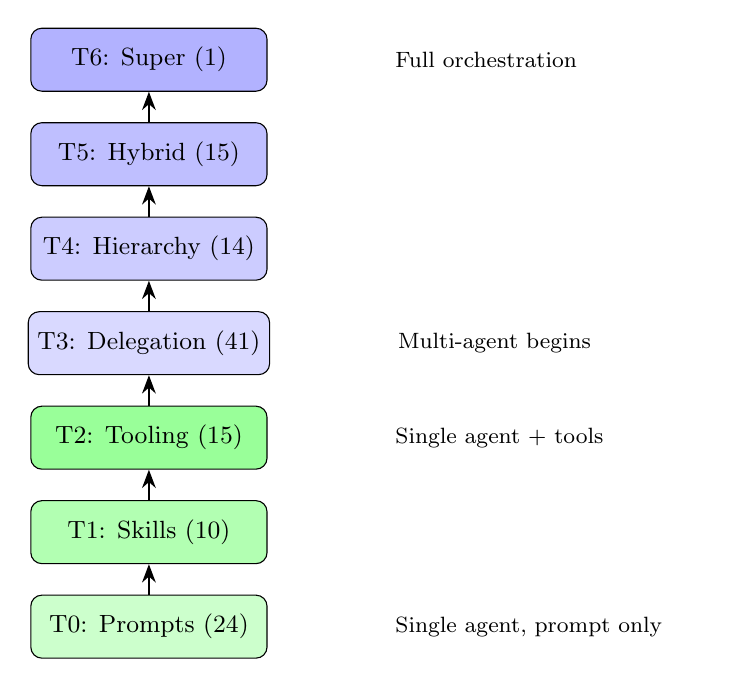
\begin{tikzpicture}[
    tier/.style={draw, rounded corners, minimum width=3cm, minimum height=0.8cm,
      font=\small},
    >=Stealth
  ]
    \node[tier, fill=green!20]  (t0) at (0,0)    {T0: Prompts (24)};
    \node[tier, fill=green!30]  (t1) at (0,1.2)  {T1: Skills (10)};
    \node[tier, fill=green!40]  (t2) at (0,2.4)  {T2: Tooling (15)};
    \node[tier, fill=blue!15]    (t3) at (0,3.6)  {T3: Delegation (41)};
    \node[tier, fill=blue!20]    (t4) at (0,4.8)  {T4: Hierarchy (14)};
    \node[tier, fill=blue!25]    (t5) at (0,6.0)  {T5: Hybrid (15)};
    \node[tier, fill=blue!30]    (t6) at (0,7.2)  {T6: Super (1)};

    \draw[->, thick] (t0) -- (t1);
    \draw[->, thick] (t1) -- (t2);
    \draw[->, thick] (t2) -- (t3);
    \draw[->, thick] (t3) -- (t4);
    \draw[->, thick] (t4) -- (t5);
    \draw[->, thick] (t5) -- (t6);

    \node[right=1.5cm of t0, font=\footnotesize, text width=4cm]
      {Single agent, prompt only};
    \node[right=1.5cm of t2, font=\footnotesize, text width=4cm]
      {Single agent + tools};
    \node[right=1.5cm of t3, font=\footnotesize, text width=4cm]
      {Multi-agent begins};
    \node[right=1.5cm of t6, font=\footnotesize, text width=4cm]
      {Full orchestration};
  \end{tikzpicture}
  \caption{Scylla tier hierarchy. Green tiers (T0--T2) represent single-agent
    configurations; blue tiers (T3--T6) introduce multi-agent coordination.
    All tiers achieve comparable pass rates (0.935--1.000) in this study.}
  \label{fig:tier_architecture}
\end{figure}

\subsection{Evaluation Protocol}
\label{sec:eval_protocol}

Each subtest defines a coding task with explicit success criteria. The Scylla
evaluation protocol proceeds as follows:

\begin{enumerate}
  \item \textbf{Configuration.} The agent receives the architectural
    configuration defined by the tier and subtest, including system prompt
    content, skill definitions, tool access, and delegation/hierarchy
    parameters.
  \item \textbf{Task Specification.} The agent receives a task description,
    target repository, and success criteria. The task specification is
    identical across all tiers for a given experiment.
  \item \textbf{Execution.} The agent executes the task using the Claude Code
    CLI~\cite{anthropic2024claude}, producing code changes, documentation,
    and/or configuration modifications. Execution is bounded by a timeout
    to prevent runaway sessions.
  \item \textbf{Evaluation.} A three-judge panel evaluates the output against
    predefined criteria. Each judge independently evaluates the output
    against weighted criteria, producing a per-judge score on a $[0, 1]$
    scale (see Section~\ref{sec:judge_panel} for details).
  \item \textbf{Consensus.} The consensus score is computed as the arithmetic
    mean of the three judge scores. Implementation rate uses the median across
    judges.
  \item \textbf{Classification.} A run is classified as ``passing'' if a
    majority of the judge panel independently classifies it as passing based
    on their individual evaluations.\footnote{The pass classification uses
    majority vote over each judge's binary pass/fail decision rather than a
    threshold on the consensus score. Of 1,080 runs, 16 (1.5\%) show the
    majority-vote outcome diverging from a na\"ive consensus-score $> 0.5$
    threshold---for example, a run with consensus score 0.487 passes because
    two of three judges passed individually, while a run with consensus score
    0.635 fails because only one of the two judges whose evaluations were
    available for that run classified it as passing (the third judge's
    evaluation was missing). These discrepancies do not materially affect
    tier-level pass rates.}
\end{enumerate}

\subsection{Partial-Failure Semantics}
\label{sec:partial_failure}

A key design decision in Scylla is its partial-failure model. When multiple
tiers run in parallel within an experiment, a tier failure does not abort the
experiment. The experiment continues with the remaining tiers and can reach a
``complete'' state even if some tiers are in a ``failed'' state. Each tier's
results are recorded independently, preserving partial results for analysis
even when individual configurations encounter infrastructure errors.
Operators must therefore check per-tier states rather than the overall
experiment state to determine whether all tiers succeeded.

\subsection{Metrics}
\label{sec:metrics}

Scylla evaluates agent performance across three categories of metrics:

\textbf{Quality Metrics.} Pass Rate ($R_{\text{pass}}$) measures the fraction
of runs exceeding the pass threshold. Implementation Rate ($R_{\text{impl}}$)
measures the proportion of rubric points achieved versus the maximum available,
using the median across judges.\footnote{Implementation rate is computed per
judge as $\sum \text{achieved}_i / \sum \text{max}_i$ across all criteria $i$
in that judge's evaluation, then the consensus uses the median across judges.
In one run (test-001, T1, subtest~01, run~1), a budget-model judge
(Haiku) assigned 4~points on a 3-point code quality criterion, producing a
per-judge implementation rate of 1.071. Combined with a missing Opus
evaluation for that run (leaving only two judges), the median implementation
rate is 1.028---the only value exceeding~1.0 in the dataset. This anomaly
does not materially affect any aggregate statistics.}
The Fine-Grained Progress Rate captures partial task completion on a continuous
scale.

\textbf{Economic Metrics.} Cost-of-Pass (CoP) is defined as the mean cost per
run divided by the pass rate:
\begin{equation}
  \text{CoP} = \frac{\overline{C}}{R_{\text{pass}}}
  \label{eq:cop}
\end{equation}
where $\overline{C}$ is the mean cost per run (in USD) and $R_{\text{pass}}$
is the pass rate. CoP captures the expected cost to obtain a passing result,
penalizing both expensive runs and low pass rates. When $R_{\text{pass}} = 0$,
CoP is undefined (infinity), indicating that no amount of spending produces a
successful outcome. Token Distribution tracks the breakdown of costs across
input, output, cache read, and cache creation operations.

\textbf{Process Metrics.} Duration measures wall-clock execution time.
Consistency captures the coefficient of variation of scores within a subtest,
measuring reproducibility. Strategic Drift measures deviation from task
objectives over the course of execution.

% ===================================================================
% 4. EXPERIMENTAL DESIGN
% ===================================================================
\section{Experimental Design}
\label{sec:experimental_design}

\subsection{Model Selection}
\label{sec:model_selection}

I select \texttt{claude-haiku-4-5} as the subject model for all experiments.
Haiku 4.5 is Anthropic's budget frontier model---the most cost-efficient
option in the Claude model family, positioned below Sonnet and Opus in the
capability hierarchy. It is designed for high-throughput, low-cost inference
while maintaining sufficient capability for coding tasks.

This selection is motivated by three considerations. First, budget models are
the most likely to be deployed at scale in production environments, making
their architectural sensitivities practically important for deployment
decisions. Second, the prior Scylla dryrun~\cite{scylla2026dryrun} used Claude
Sonnet 4.5, enabling cross-model comparison in future work. Third, the lower
per-token cost of Haiku (\$1.00/MTok input, \$5.00/MTok output for standard
pricing, with prompt caching at \$1.25/MTok for cache writes and \$0.10/MTok
for cache reads)\footnote{Anthropic pricing retrieved April 2026;
prices are subject to change.} enables a larger experimental matrix at a fixed budget.

\subsection{Task Selection}
\label{sec:task_selection}

I design three experiments of varying difficulty and domain to test the
generality of tier effects across task characteristics:

\begin{description}
  \item[test-001: Python Hello World] A trivial Python task requiring the
    creation of a ``Hello World'' program in the Hello-World repository. This
    task serves as a floor calibration: any functional agent architecture
    should achieve near-perfect performance, so the minimal complexity makes
    it a sensitive detector of architectural overhead---if a tier cannot solve
    this task, the failure is attributable to the architecture, not to task
    difficulty.
  \item[test-002: Mojo Hello World with Bazel and Documentation] A moderate
    task in the Mojo programming language, requiring a ``Hello World'' program
    within the official Modular repository together with Bazel build
    configuration and accompanying documentation. The unfamiliar language and
    complex build system have limited representation in the model's training
    data, so this task is expected to differentiate tiers and expose capability
    gaps for configurations with limited tooling or domain knowledge support.
  \item[test-003: Add mypy to pixi Configuration] A moderate Python/Mojo
    task in the ProjectOdyssey repository, requiring the addition of mypy
    type checking to an existing pixi-managed
    project~\cite{projectodyssey}. Modifying an established configuration
    tests integration capability---the agent must understand project context,
    dependency relationships, and tooling conventions, so this task is
    expected to favor tiers with richer contextual support.
\end{description}

The three tasks were selected to span a range of dimensions: language
familiarity (Python vs.\ Mojo), task type (greenfield creation vs.\
configuration modification), and repository complexity (minimal vs.\ full
project structure). While all three tasks are relatively simple by software
engineering standards, they provide sufficient variation to test whether tier
effects are task-dependent.

\subsection{Experimental Configuration}
\label{sec:exp_config}

Each experiment executes all 120 subtests across all seven tiers (T0--T6) with
$N=3$ replications per subtest. The total experiment matrix is:

\begin{itemize}
  \item 3 experiments $\times$ 120 subtests $\times$ 3 runs = 1,080 total runs
  \item 7 tiers: T0 (24 subtests), T1 (10), T2 (15), T3 (41), T4 (14),
    T5 (15), T6 (1)
  \item Subject model: \texttt{claude-haiku-4-5} (all tiers, all experiments)
  \item Judge panel: \texttt{claude-opus-4-6}, \texttt{claude-sonnet-4-6},
    \texttt{claude-haiku-4-5}
  \item Runs per subtest per experiment: $N=3$
\end{itemize}

The per-tier sample sizes across all three experiments are: T0 ($n=216$),
T1 ($n=90$), T2 ($n=135$), T3 ($n=369$), T4 ($n=126$), T5 ($n=135$),
T6 ($n=9$). The unequal sample sizes reflect the varying number of subtests
per tier, which in turn reflects the varying combinatorial complexity of each
architectural category.

\begin{table}[htbp]
\centering
\caption{Experiment Configuration (Data-Derived)}
\label{tab:experiment_config}
\small
\begin{tabular}{lrllrrr}
\toprule
Experiment & Tiers & Tier IDs & ST/Tier & Runs/ST & Total & Judges \\
\midrule
test-001 & 7 & T0, T1, T2, T3, T4, T5, T6 & 1-41 & 3 & 360 & N/A \\
test-002 & 7 & T0, T1, T2, T3, T4, T5, T6 & 1-41 & 3 & 360 & N/A \\
test-003 & 7 & T0, T1, T2, T3, T4, T5, T6 & 1-41 & 3 & 360 & N/A \\
\bottomrule
\end{tabular}
\end{table}


\subsection{Judge Panel Design}
\label{sec:judge_panel}

Evaluation uses a three-judge panel spanning the full Anthropic model
hierarchy:

\begin{enumerate}
  \item \textbf{Judge~1}: \texttt{claude-opus-4-6} --- the frontier model with
    the highest capability, serving as the most authoritative evaluator.
  \item \textbf{Judge~2}: \texttt{claude-sonnet-4-6} --- a mid-tier model
    providing an intermediate evaluation perspective.
  \item \textbf{Judge~3}: \texttt{claude-haiku-4-5} --- the budget model,
    identical to the subject agent, enabling analysis of self-evaluation bias.
\end{enumerate}

The consensus score is computed as the arithmetic mean of the three judges'
scores. Implementation rate uses the median across judges' binary assessments
of task attempt. This panel design was chosen to provide evaluation diversity
while enabling analysis of the relationship between judge capability and
evaluation reliability.

The inclusion of the subject model (Haiku) as one of its own judges is a
deliberate design choice. It enables me to test for self-preference bias
(whether the model rates its own outputs more or less favorably than external
judges) and to assess whether budget models possess sufficient evaluative
capacity to serve as reliable judges.

Each judge receives a structured evaluation prompt containing four components:
(1)~the original task prompt issued to the agent, (2)~the agent's code output
(files created or modified), (3)~build pipeline results (compilation status,
test outcomes, linting output), and (4)~a structured rubric defining five
evaluation criteria with associated weights. The criteria and their weights are:
\emph{functional correctness} (0.35), \emph{code quality} (0.20),
\emph{build pipeline} (0.10), \emph{proportionality} (0.15), and
\emph{overall quality} (0.20). Each judge scores every criterion on a 0--10
scale; the weighted sum produces a single per-judge score, and the consensus
score is the arithmetic mean across the three judges.

In practice, the number and naming of criteria varies across experiments and
judges. test-001 (Python Hello World) consistently produces the standard
five-criterion rubric across all judge evaluations. test-002 (Mojo with Bazel),
however, elicits task-specific criteria from the judges: individual evaluations
contain between 4 and 12 scored dimensions, with criterion names reflecting
Mojo-specific concerns (e.g., \emph{memory\_safety}, \emph{mojo\_syntax},
\emph{deprecated\_patterns}). test-003 (mypy configuration) collapses to
predominantly single-criterion evaluations. This variability arises because the
judge models interpret the rubric prompt with varying granularity depending on
task complexity. The per-judge score and implementation rate are computed from
whatever criteria the judge produces, so the aggregate metrics remain
well-defined even when the underlying rubric structure differs. However, the
per-criterion analysis in Table~\ref{tab:criteria_performance} is restricted to
the five standard criteria and therefore reflects primarily test-001 data.

This study's judge panel represents an architectural change from the prior
Scylla dryrun~\cite{scylla2026dryrun}. The dryrun used Claude Sonnet~4.5 as
the subject model with 4.5-series judges (Opus~4.5, Sonnet~4.5, Haiku~4.5).
The present study upgrades to 4.6-series judges---Opus~4.6 and
Sonnet~4.6---while retaining Haiku~4.5 as both subject and judge. This creates
a mixed-generation judge panel in which two judges (Opus~4.6 and Sonnet~4.6)
belong to a newer model generation than the subject agent (Haiku~4.5). The
generational gap may introduce evaluation asymmetries: newer judges may have
improved calibration or different scoring baselines relative to the subject's
generation. I note this design limitation and examine judge-level score
distributions in Section~\ref{sec:agreement_results} to assess whether
generational differences materially affect evaluation reliability.

\subsection{Statistical Methods}
\label{sec:statistical_methods}

Analysis of Variance (ANOVA) is a family of statistical tests that partition
observed variance into components attributable to different factors. Because my
data violates ANOVA's normality assumptions (Appendix~\ref{app:normality}), I
employ non-parametric alternatives throughout.

All score distributions are tested for normality using the Shapiro--Wilk test.
Of 14 tier $\times$ \{Score, Cost\} combinations, 13 reject normality
($p < 0.05$; the sole exception is T6 Cost with $n=9$, $p=0.069$; see
Appendix~\ref{app:normality}), so I employ non-parametric methods
throughout. Additional metrics (implementation rate, duration) were also
tested and similarly reject normality for most tier combinations.

The following subsections detail each statistical method used in this study,
including the test statistic, assumptions, and interpretation guidelines.

\subsubsection{Shapiro--Wilk Test}
\label{sec:shapiro_wilk}

The Shapiro--Wilk test~\cite{shapiro1965analysis} assesses whether a sample is
drawn from a normally distributed population. The test statistic is:
\begin{equation}
  W = \frac{\left(\sum_{i=1}^{n} a_i x_{(i)}\right)^2}{\sum_{i=1}^{n}(x_i - \bar{x})^2}
\end{equation}
where $x_{(i)}$ are the order statistics and $a_i$ are tabulated constants
derived from the expected values of normal order statistics. $W$ ranges from
0 to 1, with values near 1 indicating normality.

I use the Shapiro--Wilk test as a gatekeeper: when normality is rejected
($p < 0.05$), I employ non-parametric alternatives for all subsequent
analyses. This test was chosen over the Anderson--Darling and
Kolmogorov--Smirnov alternatives because of its superior power for small to
moderate sample sizes~\cite{razali2011power}, which matches my per-tier
sample sizes ($n = 9$ to $n = 369$). In this study, 13 of 14 tier $\times$
\{Score, Cost\} combinations reject normality (the sole exception is T6 Cost,
$n=9$, $p=0.069$), motivating the use of non-parametric methods throughout.

\subsubsection{Kruskal--Wallis H Test}
\label{sec:kruskal_wallis}

The Kruskal--Wallis $H$ test~\cite{kruskal1952use} is a non-parametric analog
of one-way ANOVA that tests whether $k$ independent samples originate from the
same distribution. The test statistic is:
\begin{equation}
  H = \frac{12}{N(N+1)} \sum_{j=1}^{k} n_j \left(\bar{R}_j - \bar{R}\right)^2
\end{equation}
where $N$ is the total number of observations, $n_j$ is the sample size for
group $j$, $\bar{R}_j$ is the mean rank within group $j$, and $\bar{R} =
(N+1)/2$ is the overall mean rank. Under the null hypothesis of identical
distributions, $H$ follows a $\chi^2$ distribution with $k-1$ degrees of
freedom.

I use the Kruskal--Wallis test as the omnibus test for overall tier
differences across all seven tiers ($k = 7$). Unlike one-way ANOVA, it does
not assume normality or equal variances---it requires only that the
observations be ordinal and the groups independent. A significant result
($p < 0.05$) indicates that at least one tier's distribution differs from the
others but does not identify which pairs differ, motivating the post-hoc
pairwise comparisons described below.

\subsubsection{Mann--Whitney U Test}
\label{sec:mann_whitney}

The Mann--Whitney $U$ test~\cite{mann1947test} is a non-parametric analog of
the independent-samples $t$-test that compares two independent groups. For
samples of sizes $n_1$ and $n_2$, the $U$ statistic counts the number of
times an observation from one group precedes an observation from the other in
the combined ranking:
\begin{equation}
  U = n_1 n_2 + \frac{n_1(n_1+1)}{2} - R_1
\end{equation}
where $R_1$ is the sum of ranks assigned to the first group.

I apply the Mann--Whitney $U$ test for pairwise tier comparisons following a
significant Kruskal--Wallis result. Specifically, I test 7 planned
comparisons per metric family: the 6 adjacent tier transitions (T0 vs.\ T1,
T1 vs.\ T2, \ldots, T5 vs.\ T6) plus the endpoint comparison (T0 vs.\ T6).
The test does not assume normality or equal variances, making it appropriate
for my score and cost distributions. A significant result indicates that the
two tiers' distributions are stochastically different.

\subsubsection{Holm--Bonferroni Correction}
\label{sec:holm_bonferroni}

The Holm--Bonferroni correction~\cite{holm1979simple} is a step-down procedure
that controls the family-wise error rate (FWER) when performing multiple
hypothesis tests. Given $m$ tests with ordered $p$-values $p_{(1)} \leq
p_{(2)} \leq \cdots \leq p_{(m)}$, the procedure rejects hypothesis $(i)$ if:
\begin{equation}
  p_{(i)} \leq \frac{\alpha}{m - i + 1}
\end{equation}
starting from the smallest $p$-value and stopping at the first non-rejected
hypothesis.

I chose the Holm--Bonferroni correction over two alternatives. Compared to the
standard Bonferroni correction ($\alpha/m$ for all tests), Holm--Bonferroni is
uniformly more powerful while still controlling FWER at level $\alpha$. Compared
to the Benjamini--Hochberg procedure~\cite{benjamini1995controlling}, which
controls the false discovery rate (FDR), Holm--Bonferroni provides stronger
error control by bounding the probability of \emph{any} false rejection rather
than the expected \emph{proportion} of false rejections. Given my small number
of planned comparisons ($m = 7$), the power loss relative to FDR control is
modest, and the stronger FWER guarantee is preferable for confirmatory analysis.

\subsubsection{Cliff's Delta}
\label{sec:cliffs_delta}

Cliff's $\delta$~\cite{cliff1993dominance} is a non-parametric effect size
measure that quantifies the degree of overlap between two distributions. It is
defined as:
\begin{equation}
  \delta = \frac{\left|\{(x_i, y_j) : x_i > y_j\}\right| -
                  \left|\{(x_i, y_j) : x_i < y_j\}\right|}{n_1 \cdot n_2}
\end{equation}
where $n_1$ and $n_2$ are the sample sizes of the two groups. The statistic
ranges from $-1$ (all values in the first group are less than all values in the
second) to $+1$ (the reverse), with 0 indicating complete overlap.

I use Cliff's $\delta$ rather than Cohen's $d$ because it does not assume
normality or equal variances, matching my non-parametric testing framework. I
report 95\% bootstrap confidence intervals alongside each estimate. Effect
magnitudes are interpreted using established thresholds~\cite{romano2006appropriate}:
$|\delta| < 0.11$ (negligible), $0.11 \leq |\delta| < 0.28$ (small),
$0.28 \leq |\delta| < 0.43$ (medium), and $|\delta| \geq 0.43$ (large).

\subsubsection{BCa Bootstrap Confidence Intervals}
\label{sec:bca_bootstrap}

The bias-corrected and accelerated (BCa) bootstrap~\cite{efron1987better}
produces confidence intervals that correct for both bias and skewness in the
bootstrap distribution. Given $B$ bootstrap resamples, the BCa interval
adjusts the percentile boundaries using a bias-correction factor $\hat{z}_0$
(estimated from the proportion of bootstrap estimates below the original
statistic) and an acceleration factor $\hat{a}$ (estimated via the jackknife).

I use BCa bootstrap confidence intervals with $B = 10{,}000$ resamples for
pass rates and other proportions. The BCa method was chosen over simple
percentile bootstrap because it provides second-order accuracy---the coverage
error is $O(n^{-1})$ rather than $O(n^{-1/2})$---which is important given my
moderate sample sizes. The BCa interval is also transformation-respecting,
meaning it produces identical results regardless of the scale on which the
statistic is computed.

\subsubsection{Clopper--Pearson Intervals}
\label{sec:clopper_pearson}

The Clopper--Pearson interval~\cite{clopper1934use} is an exact confidence
interval for a binomial proportion. For $k$ successes in $n$ trials, the
$100(1-\alpha)\%$ interval is:
\begin{equation}
  \left[B\!\left(\frac{\alpha}{2};\, k,\, n-k+1\right),\;
        B\!\left(1-\frac{\alpha}{2};\, k+1,\, n-k\right)\right]
\end{equation}
where $B(p;\, a, b)$ is the $p$-th quantile of the Beta distribution with
parameters $a$ and $b$.

I use Clopper--Pearson intervals for small-sample tiers, particularly T6 with
$n = 9$ runs per experiment. Unlike the normal approximation or Wilson interval,
the Clopper--Pearson interval guarantees at least nominal coverage for any
sample size, making it the conservative choice when $n$ is too small for
asymptotic methods to be reliable. The resulting intervals are wider than
approximate alternatives, which I consider appropriate given my emphasis on
hedged conclusions.

\subsubsection{Scheirer--Ray--Hare Test}
\label{sec:srh_test}

The Scheirer--Ray--Hare (SRH) test~\cite{scheirer1976analysis} is a
non-parametric extension of two-way ANOVA that operates on ranked data. All
observations are ranked jointly, and the total sum of squared ranks is
decomposed into components attributable to each main effect and their
interaction. The test statistic for each factor is:
\begin{equation}
  H_{\text{factor}} = \frac{SS_{\text{factor}}}{SS_{\text{total}} / (N-1)}
\end{equation}
which is compared against a $\chi^2$ distribution with degrees of freedom
equal to those of the corresponding factor.

I use the SRH test to assess tier $\times$ experiment interactions---that is,
whether the effect of architectural tier varies across tasks. This is critical
for determining whether a single ``best tier'' exists or whether the optimal
configuration is task-dependent. The SRH test decomposes effects into three
components: the tier main effect, the experiment main effect, and the
tier $\times$ experiment interaction. A significant interaction term indicates
that tier rankings are not stable across experiments. I note that the
validity of the SRH interaction test has been debated in the
literature~\cite{scheirer1976analysis}, and the test's power may be limited
for unbalanced designs. The interaction results should therefore be
interpreted as directional evidence rather than definitive conclusions.

\subsubsection{Krippendorff's Alpha}
\label{sec:krippendorffs_alpha}

Krippendorff's $\alpha$~\cite{krippendorff2004content} measures inter-rater
reliability for any number of raters, any number of categories, and any level
of measurement. It is defined as:
\begin{equation}
  \alpha = 1 - \frac{D_o}{D_e}
\end{equation}
where $D_o$ is the observed disagreement among raters and $D_e$ is the
disagreement expected by chance. For interval-scale data (as used here), the
difference function is squared Euclidean distance between values.

I use Krippendorff's $\alpha$ on the interval scale to assess overall
agreement among the three-judge panel. It was chosen over alternatives such as
Cohen's $\kappa$ (limited to two raters and nominal data) and the intraclass
correlation coefficient (assumes normality) because it handles missing data
natively, supports any number of raters, and is appropriate for interval-scale
scores. Interpretation follows established thresholds~\cite{krippendorff2004content}:
$\alpha < 0.667$ is unacceptable for drawing conclusions, $0.667 \leq \alpha
< 0.800$ permits tentative conclusions, and $\alpha \geq 0.800$ indicates
acceptable reliability. I supplement $\alpha$ with pairwise Spearman and
Pearson correlations to diagnose which judge pairs contribute most to
agreement or disagreement.

Implementation rate comparisons use filtered sample sizes: only runs where the
agent attempted the task contribute to the pairwise tests, which reduces the
effective $n$ for some tiers relative to the full run count.

Given the small sample size ($N=3$ per subtest), all confidence intervals are
necessarily wide. I adopt hedged language throughout and characterize my
findings as preliminary evidence rather than definitive conclusions. The
results should be interpreted as directional signals that motivate
larger-scale confirmation studies.

% ===================================================================
% 5. RESULTS
% ===================================================================
\section{Results}
\label{sec:results}

\subsection{Experiment Overview}
\label{sec:experiment_overview}

Table~\ref{tab:experiment_overview} presents the high-level results for each
experiment. All three experiments achieve high aggregate pass rates, ranging
from 0.950 (test-002) to 0.992 (test-001), with total costs ranging from
\$14.71 to \$81.28.

\input{tables/tab11_experiment_overview}

The trivial task (test-001) achieves the \emph{highest} overall pass rate
(0.992), consistent with the expectation that simpler tasks are solved more
reliably. test-003 (mypy configuration) follows at 0.956, and test-002 (Mojo
with Bazel) achieves 0.950---the lowest pass rate but the highest cost,
reflecting the greater complexity of producing unfamiliar-language code with
build configuration.

The best tier varies across experiments: T1 for test-001, T6 for test-002 and
test-003 (though T6 has only $n=3$ runs per experiment and very wide confidence
intervals; see Section~\ref{sec:cross_task}). This variation provides an initial
indication that the optimal architectural configuration is task-dependent, a
finding I formalize through
interaction analysis in Section~\ref{sec:interaction}.

Figure~\ref{fig:tier_summary_heatmap} provides an overview of score
distributions across all tiers and experiments.

\begin{figure}[htbp]
  \centering
  \includegraphics[width=\textwidth]{fig15c_tier_summary_heatmap.png}
  \caption{Tier summary heatmap showing mean consensus scores by tier (y-axis)
    and run number (x-axis). Color encodes mean score
    (red--yellow--green scale). All tiers show predominantly green cells,
    indicating consistently high scores across architectural configurations.}
  \label{fig:tier_summary_heatmap}
\end{figure}

\subsection{test-001: Python Hello World}
\label{sec:test001}

The trivial Python Hello World task achieves near-perfect performance across
all tiers, with an aggregate pass rate of 0.992. The per-tier results
confirm that the task's simplicity makes it solvable by every architectural
configuration:

\begin{table}[htbp]
  \centering
  \caption{test-001 (Python Hello World): Per-tier results. All tiers achieve
    pass rates above 0.95, consistent with the trivial nature of the task.}
  \label{tab:test001}
  \small
  \begin{tabular}{lrrrrr}
    \toprule
    Tier & $n$ & Pass Rate & Score & Cost/Run (\$) & CoP (\$) \\
    \midrule
    T0 & 72  & 0.958 & 0.870 & 0.038 & 0.040 \\
    T1 & 30  & 1.000 & 0.908 & 0.037 & 0.037 \\
    T2 & 45  & 1.000 & 0.908 & 0.037 & 0.037 \\
    T3 & 123 & 1.000 & 0.928 & 0.041 & 0.041 \\
    T4 & 42  & 1.000 & 0.927 & 0.044 & 0.044 \\
    T5 & 45  & 1.000 & 0.930 & 0.042 & 0.042 \\
    T6 & 3   & 1.000 & 0.930 & 0.106 & 0.106 \\
    \bottomrule
  \end{tabular}
\end{table}

The near-universal success on this trivial task establishes an important
baseline: for a task requiring only a single line of code
(\texttt{print("Hello, World!")}), no significant effect of architectural
complexity on performance was detected. All delegation-based tiers (T3--T6)
achieve perfect pass rates, suggesting that coordination overhead did not
detectably impede the budget model on simple tasks.

T1 and T2 achieve perfect pass rates (1.000) with identical scores (0.908),
suggesting that skills and tooling provide no marginal benefit over basic
prompts for this trivial task, but also introduce no overhead. T0 achieves a
slightly lower pass rate (0.958), indicating that some prompt configurations
in the T0 ablation spectrum (particularly minimal or empty prompts) cause
occasional failures.

Inspection of the per-subtest data reveals that the T0 failures on test-001
are concentrated in subtest~00, the empty-prompt configuration
(\texttt{system\_prompt\_mode: none}). With subtest~00 excluded, T0 achieves a
perfect 1.000 pass rate on test-001, identical to all other tiers. The
empty-prompt agent receives the task instructions as a user message but has no
system prompt providing behavioral framing. Examination of the agent
transcripts reveals that rather than executing the task, the model
meta-reasons about the evaluation framework---describing what the task asks
for and posing clarifying questions (``Would you like me to execute this
task?'')---completing in only 2~API calls and $\sim$6\,s of agent time. In
contrast, subtest~01 (which adds only the default tool system prompt) executes
the task immediately and succeeds. This suggests that the system prompt's role
is not merely informational but \emph{behavioral}: it provides the framing
that shifts a budget model from meta-reasoning to task execution, even when
the task instructions are unambiguous.

The cost per run is low across all tiers (\$0.037--\$0.106), confirming that
on trivial tasks the agent consumes modest resources regardless of
architectural configuration. The elevated cost for T6 (\$0.106) reflects the
overhead of the full-capability configuration, though this does not translate
into any quality advantage on a task that all simpler tiers already solve
perfectly.

\subsection{test-002: Mojo Hello World with Bazel and Documentation}
\label{sec:test002}

The moderate Mojo task achieves high pass rates across all tiers, with
modest differentiation across the architectural spectrum:

\begin{table}[htbp]
  \centering
  \caption{test-002 (Mojo Hello World): Per-tier results. All tiers achieve
    pass rates above 0.90, with modest variation.}
  \label{tab:test002}
  \small
  \begin{tabular}{lrrrrr}
    \toprule
    Tier & $n$ & Pass Rate & Score & Cost/Run (\$) & CoP (\$) \\
    \midrule
    T0 & 72  & 0.903 & 0.641 & 0.219 & 0.242 \\
    T1 & 30  & 0.933 & 0.676 & 0.229 & 0.245 \\
    T2 & 45  & 0.956 & 0.685 & 0.222 & 0.232 \\
    T3 & 123 & 0.967 & 0.686 & 0.229 & 0.237 \\
    T4 & 42  & 0.976 & 0.677 & 0.236 & 0.242 \\
    T5 & 45  & 0.956 & 0.694 & 0.217 & 0.228 \\
    T6 & 3   & 1.000 & 0.722 & 0.279 & 0.279 \\
    \bottomrule
  \end{tabular}
\end{table}

For this task, pass rates increase slightly from T0 (0.903) to T6 (1.000),
with a modest upward trend suggesting that additional architectural
capabilities provide marginal benefit on more complex tasks. This
task-dependent tier profile is a key driver of the significant tier $\times$
experiment interaction discussed in Section~\ref{sec:interaction}.

Scores cluster between 0.641 and 0.722, suggesting that while the agent
consistently attempts and partially completes the task, the quality ceiling is
bounded by factors other than architecture---likely the model's familiarity
with Mojo syntax and Bazel build system configuration. The relatively narrow
score range (0.081 span) indicates that the task difficulty, rather than the
architecture, is the primary determinant of output quality.

The Cost-of-Pass is remarkably uniform across tiers (\$0.228--\$0.279),
consistent with the aggregate cost invariance finding. T6 ($n=3$) achieves the
highest pass rate (1.000) but at the highest CoP (\$0.279), reflecting its
elevated per-run cost.

One interpretation of these results is that the Mojo task's complexity
provides sufficient ``work'' to leverage the coordination capabilities of
delegation-based tiers. The Mojo task involves multiple components (source
code, build configuration, documentation) that can genuinely benefit from
decomposition. A complementary explanation is that the model's limited
familiarity with Mojo---noted in Section~\ref{sec:task_selection} as having
``limited representation in the model's training data''---means that specialist
agents in delegation-based tiers may provide language-specific context or
tooling that partially compensates for the base model's limited training
exposure. This advantage is absent for well-represented languages like Python,
where the base model already possesses deep knowledge.

\subsection{test-003: Add mypy to pixi Configuration}
\label{sec:test003}

The mypy configuration task shows uniformly high pass rates with subtle tier
effects:

\begin{table}[htbp]
  \centering
  \caption{test-003 (Add mypy to pixi): Per-tier results. High pass rates
    across all tiers with modest variation.}
  \label{tab:test003}
  \small
  \begin{tabular}{lrrrrr}
    \toprule
    Tier & $n$ & Pass Rate & Score & Cost/Run (\$) & CoP (\$) \\
    \midrule
    T0 & 72  & 0.944 & 0.817 & 0.071 & 0.076 \\
    T1 & 30  & 0.967 & 0.865 & 0.074 & 0.076 \\
    T2 & 45  & 0.978 & 0.814 & 0.073 & 0.074 \\
    T3 & 123 & 0.959 & 0.826 & 0.071 & 0.074 \\
    T4 & 42  & 0.952 & 0.857 & 0.076 & 0.080 \\
    T5 & 45  & 0.933 & 0.829 & 0.098 & 0.105 \\
    T6 & 3   & 1.000 & 0.833 & 0.100 & 0.100 \\
    \bottomrule
  \end{tabular}
\end{table}

Pass rates are uniformly high (0.933--1.000) with no clear monotonic trend.
Scores range from 0.814 to 0.865, with T1 (skills) achieving the highest
score (0.865). This suggests that for configuration tasks, domain-specific
skills provide marginally more benefit than raw tool access or delegation,
possibly because skills contain procedural knowledge about configuration
management that the base model does not possess.

An interesting anomaly is T5 (hybrid), which shows elevated cost
(\$0.098/run vs.\ \$0.071--\$0.076 for T0--T3) without a corresponding
quality improvement (pass rate 0.933 is the lowest in the table). The hybrid
configurations appear to introduce overhead from combining multiple
architectural elements without the coordination benefits that might emerge
on more complex tasks.

T6 achieves a perfect pass rate (1.000) but with only $n=3$ runs, this
result should be interpreted with extreme caution. At the aggregate level
($n=9$ across three experiments), T6's pass rate is 1.000. The
Clopper--Pearson exact 95\% confidence interval~\cite{clopper1934use}
$[0.664, 1.000]$ still admits substantial uncertainty at this sample size,
and the true pass rate could be considerably lower.

\subsection{Cross-Task Analysis}
\label{sec:cross_task}

Aggregating across all three experiments, Table~\ref{tab:tier_summary}
presents the tier-level summary statistics.

\input{tables/tab01_tier_summary}

The aggregate results reveal a remarkably uniform performance profile across
all tiers. Pass rates range from 0.935 (T0) to 1.000 (T6), with scores
clustered between 0.776 and 0.828. No sharp performance boundary exists
between single-agent tiers (T0--T2) and delegation-based tiers (T3--T6);
instead, all tiers perform well, with T0 showing slightly lower pass rates
and consistency than the remaining tiers.

\begin{figure}[htbp]
  \centering
  \includegraphics[width=\textwidth]{fig04_pass_rate_by_tier.png}
  \caption{Score distributions per tier (histogram, bin width 0.05). Each
    panel shows the distribution of per-run consensus scores for one tier.
    The red dashed vertical line marks the pass threshold. All tiers show
    distributions concentrated at high scores, with T0 exhibiting slightly
    greater spread.}
  \label{fig:pass_rate_by_tier}
\end{figure}

Tier-level consistency ($1 - \text{CV}$, computed over all runs in each tier)
ranges from 0.734 (T0) to 0.841 (T6) in Table~\ref{tab:tier_summary},
indicating that all tiers produce reasonably reproducible outcomes at the
aggregate level. However, per-subtest consistency (computed independently for
each subtest and then averaged) shows wider variation, with some tiers
exhibiting lower reproducibility at the subtest level---notably T5, whose
hybrid configurations produce inconsistent results on individual subtests
despite adequate aggregate performance. The modest consistency advantage of
T1--T6 over T0 may reflect the stabilizing effect of additional architectural
scaffolding (skills, tools, or delegation protocols) that reduces sensitivity
to prompt variation.

\begin{figure}[htbp]
  \centering
  \includegraphics[width=\textwidth]{fig01_score_variance_by_tier.png}
  \caption{Score distributions by tier. All tiers show similar variance
    profiles, with the majority of scores concentrated at high values.
    T0 exhibits modestly greater spread, consistent with its wider range
    of prompt configurations.}
  \label{fig:score_variance}
\end{figure}

The Kruskal--Wallis omnibus test reveals \emph{no} significant tier effects
for pass rate, implementation rate, or duration:

\begin{itemize}
  \item Pass rate: $H(6) = 8.53$, $p = 0.2015$ (not significant)%
    \footnote{For the binary pass/fail outcome, a chi-squared test on the
    $2 \times 7$ contingency table would be the more natural choice. I use
    Kruskal--Wallis throughout for a unified analytical framework; the
    conclusions are qualitatively identical under both tests.}
  \item Score: $H(6) = 91.3$ (from SRH tier factor), $p < 0.001$ (significant)
  \item Duration: $H(6) = 6.74$, $p = 0.345$ (not significant)
  \item Cost: $H(6) = 4.00$, $p = 0.676$ (not significant)
  \item Implementation rate: $H(6) = 5.83$, $p = 0.4423$ (not significant)
\end{itemize}

Note that the Score and Cost tier statistics above are drawn from the
Scheirer--Ray--Hare tier main effect (Section~\ref{sec:interaction}), as the
omnibus pipeline tests only pass rate, implementation rate, and duration
directly.

The non-significance of pass rate, cost, implementation rate, and duration
across tiers is the central finding of this study. It means that all tiers
achieve statistically indistinguishable pass rates, cost approximately the
same, exhibit similar implementation rates, and complete in comparable time.
The only metric showing a significant tier effect is the continuous
\emph{score}, which captures finer-grained quality differences within the
predominantly passing runs. Since the omnibus test for pass rate is not
significant, no pairwise comparisons are warranted.

The non-significance of pass rate is best read as a ceiling-effect artifact:
the three tasks selected here are well within the model's demonstrated
capability, so every architectural tier converges on near-perfect pass rates
with little room to differentiate. More demanding tasks---multi-file
refactors, cross-repository changes, or problems the model has not previously
solved---would likely re-expose the architectural differences that this study
could not detect at the pass-rate level, and replication on harder benchmarks
may yield a different result.

\begin{figure}[htbp]
  \centering
  \includegraphics[width=\textwidth]{fig19_effect_size_forest.png}
  \caption{Forest plot of Cliff's $\delta$ effect sizes for pairwise tier
    comparisons on score (lower-numbered tier is reference group; negative
    $\delta$ indicates the higher-numbered tier has lower scores).
    Effect sizes are uniformly small, consistent with the non-significant
    omnibus test on pass rate.
    Error bars show 95\% bootstrap confidence intervals.}
  \label{fig:effect_size_forest}
\end{figure}

\subsection{Tier $\times$ Task Interaction}
\label{sec:interaction}

The most analytically important finding is the significant tier $\times$
experiment interaction on \emph{score}. The Scheirer--Ray--Hare (SRH) test
provides a non-parametric decomposition of the effects of tier, experiment,
and their interaction on the ranked outcome variables:

\begin{table}[htbp]
  \centering
  \caption{Scheirer--Ray--Hare analysis of tier $\times$ experiment
    interactions. The score interaction ($H=223.5$) exceeds both main
    effects, indicating that tier effects on score are strongly
    task-dependent.}
  \label{tab:srh}
  \small
  \begin{tabular}{llrrcl}
    \toprule
    Metric & Factor & $H$ & df & $p$ & Sig? \\
    \midrule
    Score & Experiment   & 178.2 & 2  & $<0.001$ & *** \\
    Score & Tier         &  91.3 & 6  & $<0.001$ & *** \\
    Score & Interaction  & 223.5 & 12 & $<0.001$ & *** \\
    \midrule
    Cost  & Experiment   & 903.1 & 2  & $<0.001$ & *** \\
    Cost  & Tier         &   4.00 & 6  & 0.676    & n.s. \\
    Cost  & Interaction  &   4.79 & 12 & 0.965    & n.s. \\
    \midrule
    Impl Rate & Experiment   & 490.7 & 2  & $<0.001$ & *** \\
    Impl Rate & Tier         &   5.47 & 6  & 0.486    & n.s. \\
    Impl Rate & Interaction  &   3.66 & 12 & 0.989    & n.s. \\
    \bottomrule
  \end{tabular}
\end{table}

All three score effects are significant at $p<0.001$: the tier $\times$
experiment interaction ($H=223.5$, $df=12$), the experiment main effect
($H=178.2$, $df=2$), and the tier main effect ($H=91.3$, $df=6$). Raw
$H$-statistics are not directly comparable across terms with different degrees
of freedom, but the significance of all three effects---particularly the
interaction---indicates that the impact of architectural complexity on
\emph{score quality} is not uniform: it depends on the task being performed.

Crucially, this interaction operates on the continuous score metric, not on
pass rate. All tiers achieve high pass rates across all experiments (the
omnibus KW test on pass rate is non-significant at $p=0.2015$). The
interaction instead reflects that the \emph{relative quality ranking} of tiers
shifts across tasks. In test-001, the trivial task provides little room for
quality differentiation and all tiers score similarly at the high end. In
test-002, tiers with delegation capabilities (T3--T6) show a modest score
advantage, possibly reflecting the benefit of task decomposition for
multi-component Mojo projects. In test-003, the tier profile is relatively
flat, with T1 (skills) showing a slight score edge on the configuration task.

For cost, the experiment main effect is dominant ($H=903.1$, $p<0.001$),
reflecting the differing cost profiles of the three tasks. test-002 (Mojo) is
approximately $6\times$ as expensive per run as test-001 (Python Hello
World). However, neither the tier main effect ($H=4.00$, $p=0.676$) nor the
interaction ($H=4.79$, $p=0.965$) is significant for cost, indicating that
no significant effect of architectural complexity on expenditure was detected.

The implementation rate shows a similar pattern to cost: strong experiment
effects ($H=490.7$, $p<0.001$) but no significant tier effects or
interactions. This indicates that the agent's \emph{willingness to attempt}
the task is driven by task characteristics rather than architectural
configuration.

\begin{figure}[htbp]
  \centering
  \includegraphics[width=\textwidth]{fig36_tier_rank_stability.png}
  \caption{Tier rank stability heatmap. Each cell shows the rank of a tier
    (x-axis) within a given experiment (y-axis, sorted by difficulty), where
    rank 1 is best. Color encodes rank (green = best, red = worst). The
    changing color pattern across experiments indicates that tier rankings
    are not stable---the optimal tier varies by task, consistent with the
    significant tier $\times$ experiment interaction on score.}
  \label{fig:tier_rank_stability}
\end{figure}

Figure~\ref{fig:grade_heatmap} provides a granular view of grade distributions
across all subtests and experiments, illustrating the task-dependent patterns
that drive the interaction effect.

\begin{figure}[htbp]
  \centering
  \includegraphics[width=\textwidth]{fig05_grade_heatmap.png}
  \caption{Grade distribution heatmap. Each cell represents the proportion
    of runs assigned each letter grade for a tier--grade combination.
    The predominantly A/B grades across all tiers and
    experiments reflect the uniformly high pass rates, with subtle
    shifts in grade distribution driving the significant score interaction.}
  \label{fig:grade_heatmap}
\end{figure}

\subsection{Per-Criterion Analysis}
\label{sec:criteria}

The judge panel evaluates each run against five weighted criteria:
functional correctness, code quality, build pipeline integrity,
proportionality (response length and scope appropriateness), and overall
quality (a holistic assessment). As noted in
Section~\ref{sec:judge_panel}, the actual criteria produced by judges vary
across experiments; the analysis below is restricted to evaluations that
used the standard five-criterion rubric (predominantly test-001, with
partial coverage in test-002 and test-003).

Across the matched evaluations, the per-criterion mean scores reveal that the
budget model's weakest dimension is functional correctness
(0.891~$\pm$~0.239), while code quality (0.980~$\pm$~0.100), build pipeline
integrity (0.965~$\pm$~0.112), and proportionality (0.964~$\pm$~0.099) score
substantially higher. Overall quality averages 0.926~$\pm$~0.099. This
pattern---high marks on surface quality but lower marks on functional
correctness---is consistent with the hypothesis that the budget model produces
syntactically well-formed code that occasionally fails to satisfy the task's
functional requirements.

% ===================================================================
% 6. INTER-RATER RELIABILITY
% ===================================================================
\section{Inter-Rater Reliability}
\label{sec:interrater}

\subsection{Panel Design}
\label{sec:panel_design}

The three-judge panel employs models spanning the full Anthropic capability
spectrum. Judge~1 (\texttt{claude-opus-4-6}) is the most capable model in the
lineup, Judge~2 (\texttt{claude-sonnet-4-6}) is mid-tier, and Judge~3
(\texttt{claude-haiku-4-5}) is the budget model---the same model used as the
subject agent.

This design was intentional: using the subject model as one of its own judges
enables analysis of self-evaluation bias. However, it also introduces the
risk that the budget judge may lack the evaluative capacity to distinguish
quality levels in its own outputs. The panel represents a pragmatic
compromise between evaluation cost (using only frontier judges would be
expensive) and reliability (using only budget judges might be unreliable).

\subsection{Agreement Results}
\label{sec:agreement_results}

Table~\ref{tab:judge_agreement} presents the full inter-rater reliability
statistics.

\input{tables/tab03_judge_agreement}

The headline finding is that Krippendorff's $\alpha$ (interval) is $0.034$,
computed on $N=1{,}080$ items (120 subtests $\times$ 3 runs per subtest
$\times$ 3 experiments) from the 3,210 available judge evaluations
(99.1\% of the 3,240 expected; see Section~\ref{sec:limitations} for
discussion of missing evaluations).
The resulting $\alpha = 0.034$ is barely above chance agreement ($\alpha = 0$). By conventional
standards in content analysis~\cite{krippendorff2004content, polo2024efficient}, $\alpha < 0.667$ is
considered
unacceptable for drawing conclusions about individual cases, and
$\alpha > 0.800$ is required for reliable measurement. My value of $0.034$
indicates that the three judges agree only marginally better than would be
expected by random scoring.

The near-zero value of $\alpha$ is concerning. While $\alpha = 0$
would indicate random agreement, $\alpha = 0.034$ provides essentially no
useful signal---the judges are producing nearly uncorrelated evaluations.
This could arise if the judges apply fundamentally different evaluation
criteria or if their evaluation strategies diverge (e.g., one judge favoring
verbose output while another penalizes it).

Pairwise correlations reveal a structured pattern of disagreement. Spearman
rank correlations are near zero for all pairs:

\begin{itemize}
  \item Judge~1 (Opus) vs.\ Judge~2 (Sonnet): $\rho = 0.177$
  \item Judge~1 (Opus) vs.\ Judge~3 (Haiku): $\rho = 0.111$
  \item Judge~2 (Sonnet) vs.\ Judge~3 (Haiku): $\rho = 0.084$
\end{itemize}

These weak rank correlations indicate that the judges show only marginal
agreement on the \emph{relative ordering} of outputs. An output that Opus
rates highly may be rated poorly by Sonnet or Haiku, and vice versa.

Pearson correlations are somewhat higher, suggesting some linear association
in score magnitudes:

\begin{itemize}
  \item Judge~1 (Opus) vs.\ Judge~2 (Sonnet): $r = 0.588$
  \item Judge~1 (Opus) vs.\ Judge~3 (Haiku): $r = 0.310$
  \item Judge~2 (Sonnet) vs.\ Judge~3 (Haiku): $r = 0.257$
\end{itemize}

The discrepancy between Spearman and Pearson correlations (particularly for
Opus--Sonnet: $\rho = 0.177$ vs.\ $r = 0.588$) suggests a non-linear
relationship between judge scores. The moderate Pearson correlation may
reflect shared calibration of score scale (both judges tend to use similar
score ranges) even though they disagree on which outputs deserve high vs.\
low scores.

\begin{figure}[htbp]
  \centering
  \begin{subfigure}[b]{0.48\textwidth}
    \includegraphics[width=\textwidth]{fig14_t0_judge_agreement.png}
    \caption{T0 (Prompts)}
  \end{subfigure}
  \hfill
  \begin{subfigure}[b]{0.48\textwidth}
    \includegraphics[width=\textwidth]{fig14_t3_judge_agreement.png}
    \caption{T3 (Delegation)}
  \end{subfigure}
  \caption{Judge agreement scatter plots for T0 and T3. Each point represents
    a run, with axes showing scores from different judge pairs. The wide
    scatter and lack of diagonal clustering illustrate the low inter-rater
    reliability across both simple (T0) and delegation-based (T3) tiers.}
  \label{fig:judge_agreement}
\end{figure}

\subsection{Judge Bias}
\label{sec:judge_bias}

\subsubsection{Directional Bias}

Examination of raw score distributions reveals directional scoring tendencies
across the panel. Opus (Judge~1) and Sonnet (Judge~2) tend to produce broadly
similar score levels, while Haiku (Judge~3) diverges. On tasks where the
frontier judges assign high scores, Haiku tends to score lower; conversely,
on tasks where frontier judges identify deficiencies, Haiku sometimes assigns
higher scores. This bidirectional disagreement---rather than a consistent
upward or downward bias---explains why pairwise Spearman correlations
involving Haiku are weaker ($\rho = 0.111$ and $\rho = 0.084$) than the
Opus--Sonnet pair ($\rho = 0.177$).

\subsubsection{Mean Absolute Differences}

The mean absolute score differences reveal a systematic pattern in which
disagreement scales with the capability gap between judges:

\begin{itemize}
  \item Judge~1 (Opus) vs.\ Judge~2 (Sonnet): mean $|\Delta| = 0.0738$
  \item Judge~1 (Opus) vs.\ Judge~3 (Haiku): mean $|\Delta| = 0.1683$
  \item Judge~2 (Sonnet) vs.\ Judge~3 (Haiku): mean $|\Delta| = 0.2186$
\end{itemize}

The two most capable models (Opus and Sonnet) agree most closely, with a mean
absolute difference of only 0.074 on a $[0, 1]$ scale. As the capability gap
increases, disagreement grows: Opus and Haiku disagree by 0.168, while Sonnet
and Haiku disagree most at 0.219.

\subsubsection{Capability-Gap Hypothesis}

This monotonic relationship between capability gap and disagreement is
consistent with the hypothesis that the budget model lacks sufficient
evaluative capacity to produce reliable judgments. Haiku may be applying
different evaluation criteria, assigning scores based on surface features
(e.g., output length, code structure) rather than the deeper quality
assessments (e.g., correctness, completeness, adherence to specifications)
performed by the frontier judges.

\subsubsection{Consensus Scoring and Signal Loss}

The near-zero Krippendorff's $\alpha$ raises a methodological concern that
affects the interpretation of all results in this paper. If the judges do not
agree, then the consensus score (arithmetic mean) may not be a reliable
measure of output quality. The mean of disagreeing judges produces a
compromise value that no individual judge endorses, potentially masking
genuine quality differences between tiers.

This problem is well-known in measurement theory: when raters hold
fundamentally different positions, averaging their scores produces a
compromise value that no individual rater endorses and obscures the
underlying disagreement. A consensus score of 0.7 might represent unanimous
moderate agreement---or it might represent one judge scoring 0.95 and
another scoring 0.45, a situation where the average conceals a substantive
disagreement about output quality.

The implementation rate metric already uses median-based consensus (the median
of three judges' binary assessments), which is more robust to a single
outlier judge than the arithmetic mean. Extending median-based aggregation to
continuous scores---or adopting trimmed means that exclude the most extreme
judge---may provide more robust quality measurement when inter-rater
reliability is poor. However, with only three judges, trimming reduces the
panel to a single judge, so expanding the panel size would be a prerequisite
for robust trimmed-mean approaches.

The pass rate metric (which uses majority vote over each judge's individual
binary classification) may be the most robust aggregation in this study, as
it requires only that a majority of judges agree on a pass/fail outcome
rather than precisely calibrated scores.

% ===================================================================
% 7. COST ANALYSIS
% ===================================================================
\section{Cost Analysis}
\label{sec:cost_analysis}

\subsection{Cost-of-Pass by Tier}
\label{sec:cop_by_tier}

Table~\ref{tab:cost_analysis} presents the detailed cost analysis by tier,
including mean cost per run, total cost, Cost-of-Pass, and token usage
statistics.

\input{tables/tab05_cost_analysis}

The aggregate Cost-of-Pass ranges from \$0.11 (T2) to \$0.16 (T6). This
variation is driven primarily by the denominator (pass rate) rather than the
numerator (mean cost), since mean cost per run is effectively constant across
tiers (\$0.11--\$0.16). Applying Equation~\ref{eq:cop}, the CoP for T6 is
slightly elevated because its higher mean cost (\$0.16 vs.\ \$0.11--\$0.12
for other tiers) is the primary driver, despite T6 achieving the highest
pass rate (1.000).

\begin{figure}[htbp]
  \centering
  \includegraphics[width=\textwidth]{fig06_cop_by_tier.png}
  \caption{Cost-of-Pass by tier. Each bar shows the CoP
    ($\overline{C} / R_{\text{pass}}$) for one tier. The modest variation
    reflects minor differences in pass rates rather than meaningful cost
    differences. T2 achieves the minimum CoP at \$0.11, making it the most
    cost-efficient tier in the aggregate.}
  \label{fig:cop_by_tier}
\end{figure}

T2 (Tooling) achieves the lowest aggregate CoP at \$0.11, though all tiers
fall within a narrow range (\$0.11--\$0.16). The overall pass rate of 0.966
means that most tier--experiment combinations achieve near-perfect pass rates,
compressing the CoP range. (Cost invariance is a non-significant finding under
limited power; real cost differences between tiers may exist below my ability
to detect.)

The practical implication is that, given no significant tier effect on pass
rate ($H(6)=8.53$, $p=0.2015$), the simplest tier configuration suffices.
Organizations need not invest in complex delegation or orchestration
architectures for the budget model and tasks studied here, as the additional
complexity provides no detectable benefit.

\subsection{Cost Scaling with Task Difficulty}
\label{sec:cost_scaling}

Cost varies dramatically by experiment but not by tier. The mean cost per run
ranges from \$0.04 for test-001 (trivial Python) to \$0.23 for test-002
(moderate Mojo), with test-003 (moderate Python configuration) at \$0.08.
The SRH analysis shows a highly significant experiment effect on
cost ($H(2) = 903.1$, $p < 0.001$) but no significant tier effect
($H(6) = 4.0$, $p = 0.676$).

\begin{figure}[htbp]
  \centering
  \includegraphics[width=\textwidth]{fig39_cost_scaling_with_difficulty.png}
  \caption{Cost scaling across experiments. Cost is driven primarily by task
    characteristics---repository size, language complexity, and required
    context---rather than architectural tier. The spread within each
    experiment reflects run-to-run variance, not tier differences.}
  \label{fig:cost_scaling}
\end{figure}

The cost differential between experiments is attributable to the differing
context requirements of each task. The Mojo task (test-002) requires the agent
to process a larger repository with more complex build configuration,
consuming more tokens for context. The Python Hello World task (test-001)
operates in a minimal repository, requiring minimal context.

This observed cost invariance across tiers ($p=0.676$, non-significant under
limited power) has a practical implication: if tiers indeed cost approximately
the same per run, the optimal strategy is simply to use the tier with the
highest pass rate. In the aggregate data, the Pareto frontier collapses to
a narrow region around T1--T2, though per-task analysis shows the frontier
varies (T5 dominates for test-002).

\subsection{Frontier Analysis}
\label{sec:frontier_analysis}

Figure~\ref{fig:cost_quality_pareto} presents the cost--quality Pareto
frontier across tiers, aggregated over experiments.

\begin{figure}[htbp]
  \centering
  \includegraphics[width=\textwidth]{fig08_cost_quality_pareto.png}
  \caption{Cost--quality Pareto frontier. Each point represents a tier
    (aggregated across experiments), plotted by mean cost per run (x-axis,
    log scale) and mean consensus score (y-axis). Pareto-optimal points lie
    on the upper-left frontier. The narrow spread of points reflects the
    overall high pass rate (0.966) and cost invariance across tiers.}
  \label{fig:cost_quality_pareto}
\end{figure}

The Pareto frontier is relatively flat, reflecting the high overall pass rate
(0.966) and narrow cost range across tiers. Most tier--experiment combinations
cluster in a similar region of the cost--quality space, consistent with the
non-significant tier effects on both pass rate and cost.

The total experimental cost of \$123.30 across 1,080 runs yields a mean cost
of \$0.11 per run. This shows that meaningful ablation studies can be
conducted at modest cost using budget models, making the Scylla framework
accessible for iterative evaluation during development cycles rather than
requiring dedicated evaluation budgets.

% ===================================================================
% 8. DISCUSSION
% ===================================================================
\section{Discussion}
\label{sec:discussion}

\subsection{Key Findings}
\label{sec:key_findings}

My results suggest several preliminary conclusions about the interaction
between architectural complexity and budget model performance. I organize
these findings around the four research questions posed in
Section~\ref{sec:introduction}.

\textbf{Finding 1 (RQ1): In this study, no significant tier effect on pass rate is detected.}
The Kruskal--Wallis test on pass rate yields $H(6)=8.53$, $p=0.2015$, which
does not reach significance at the $\alpha=0.05$ level. The overall pass rate
of 0.966 across all tiers indicates that the budget model performs well
regardless of architectural configuration. While individual tier--experiment
combinations show some variation, the aggregate data provide no evidence that
adding delegation, hierarchy, or hybrid configurations improves or degrades
pass rate for the tasks studied. Given the small sample size ($N=3$ per
subtest), this null result should be interpreted cautiously---real but small
tier effects may exist below my statistical power to detect.

\textbf{Finding 2 (RQ2): In this study, task-dependent effects dominate tier effects.}
The significant SRH interaction effect on score ($H(12) = 223.5$, $p < 0.001$)
is the central finding of the cross-task analysis. Both the tier main effect
($H(6) = 91.3$, $p < 0.001$) and experiment main effect ($H(2) = 178.2$,
$p < 0.001$) are significant on the continuous score metric, though their raw
$H$-values are not directly comparable across different degrees of freedom.
The highly significant interaction indicates that the \emph{combination} of
tier and task determines quality beyond either factor alone. However, this
tier effect on continuous scores does not translate to a significant effect on
the binary pass rate metric ($H(6)=8.53$, $p=0.2015$), suggesting that
score-level differences are too small to cross the pass/fail threshold
consistently.

\textbf{Finding 3 (RQ3): In this study, no significant cost variation across tiers is detected.}
Cost-of-Pass ranges from \$0.11 at T2 to \$0.16 at T6, driven by minor
differences in pass rates rather than rising per-run costs. The non-significant
tier effect on cost ($H(6) = 4.00$, $p = 0.676$) provides no evidence of a
cost--quality trade-off under current statistical power. Since neither pass
rate nor cost varies significantly by tier, the tiers are effectively
interchangeable on the tasks studied.

\textbf{Finding 4 (RQ4): In this study, the three-judge panel exhibits poor
reliability.} With Krippendorff's $\alpha = 0.034$, the judge panel produces
scores that are barely above chance agreement. The disagreement
is structured: the two frontier judges (Opus and Sonnet) show the smallest
pairwise disagreement (mean $|\Delta| = 0.074$, Spearman $\rho = 0.177$),
while the budget judge (Haiku) disagrees substantially with both
(mean $|\Delta| = 0.168$ and $0.219$). This suggests that including a budget
model in the judge panel introduces noise rather than signal, and that a
two-judge panel of frontier models might provide more reliable evaluation.

\textbf{Finding 5: Practical implication---the simplest tier suffices.} Since
no significant tier effect is detected on either pass rate or cost, the
practical recommendation is straightforward: organizations deploying the budget
model on tasks of comparable complexity should use the simplest architecture
that meets their requirements. Additional complexity (delegation, hierarchy,
hybrid configurations) provides no detectable benefit in this study and adds
operational overhead in configuration and maintenance.

\subsection{Practical Implications}
\label{sec:practical_implications}

These findings have several practical implications for organizations deploying
agentic coding systems with budget models.

\textbf{Tier equivalence favors simplicity.} Since no significant tier effect
is detected on pass rate ($p=0.2015$) or cost ($p=0.676$), the practical
recommendation is to use the simplest architecture that meets operational
requirements. For the budget model and tasks studied here, T0 (prompt-only)
achieves comparable results to T6 (everything enabled). The additional
engineering effort to configure delegation, hierarchy, and hybrid
architectures provides no detectable benefit in task success.

\textbf{Task characteristics dominate architecture.} The significant SRH
interaction effect on score ($p < 0.001$) indicates that task selection
matters more than architectural configuration. Organizations seeking to
improve agent performance should focus on task decomposition and prompt
engineering rather than architectural complexity. The variation in pass rate
across experiments (driven by task difficulty) exceeds the variation across
tiers within any single experiment.

\textbf{Judge panel composition matters.} The poor inter-rater
reliability ($\alpha = 0.034$) suggests that organizations using
LLM-as-judge evaluation should carefully consider panel composition.
Including budget models as judges introduces noise that may obscure real
quality differences. A two-judge panel of frontier models may provide more
reliable evaluation despite the higher per-evaluation cost.

\textbf{Budget models are cost-competitive for evaluation.} The total cost
of \$123.30 for 1,080 runs shows that systematic architectural
evaluation is affordable with budget models. Organizations can conduct their
own ablation studies during development cycles rather than relying on
published benchmarks that may not reflect their specific use cases.

\subsection{Comparison to Prior Work}
\label{sec:comparison_prior}

The prior Scylla dryrun~\cite{scylla2026dryrun} evaluated Claude Sonnet 4.5
on a single Hello World task. While direct comparison is limited by
differences in model, task set, and experimental scale, several contrasts
are noteworthy.

The dryrun found a pattern of degradation in higher tiers, whereas the
current study finds no significant tier effect on pass rate. This discrepancy
may reflect differences in the model under study (Sonnet 4.5 vs.\ Haiku 4.5),
the expanded task set (three experiments vs.\ one), or the increased
statistical rigor of the current design. The comparison highlights the
importance of multi-task evaluation: findings from a single task may not
generalize, and the apparent tier effects in the dryrun may have been
task-specific rather than architectural.

\subsection{Limitations}
\label{sec:limitations}

This study has several important limitations that constrain the
generalizability of my findings:

\textbf{Small sample size.} With $N=3$ replications per subtest, my
statistical power is limited. Bootstrap confidence intervals are necessarily
wide (e.g., the T6 pass rate CI spans $[0.664, 1.000]$), and individual
outlier runs can substantially influence subtest-level statistics. A formal post-hoc power analysis would help
quantify the risk of Type~II error for the null pass rate result; however,
the non-standard distribution of pass rates (bounded, heavily right-skewed)
complicates standard power calculations. The results should be treated as
preliminary evidence requiring confirmation with larger sample sizes
($N \geq 10$).

\textbf{Single model family.} All experiments use models from the Anthropic
Claude family. The findings may not generalize to other model families (e.g.,
GPT, Gemini, Llama) with different architectural assumptions, fine-tuning
strategies, or capability profiles. In particular, models that have been
specifically optimized for multi-agent coordination might show different tier
sensitivity profiles.

\textbf{Limited task diversity.} Three experiments provide limited coverage of
the task space. All three tasks are relatively simple by software engineering
standards---none involves multi-file refactoring, complex debugging, or
large-scale system design. The tier effects observed here may not hold for
more complex tasks where delegation could provide genuine coordination value
that offsets the overhead costs. Relatedly, the high pass rates across all
tiers (0.903--1.000) introduce a ceiling effect that limits statistical power
to detect tier differences on the binary pass/fail metric. The non-significant
Kruskal--Wallis result on pass rate may partly reflect this restricted range
rather than true tier equivalence.

\textbf{Judge reliability concerns.} The poor inter-rater reliability
($\alpha = 0.034$) undermines confidence in the quality scores. While the
pass rate metric (which uses majority vote) is less sensitive to score
miscalibration, the continuous score and CoP metrics may be substantially
affected by judge disagreement. All findings based on continuous scores
should be interpreted with this caveat in mind.

\textbf{Evaluation coverage.} Of the 3,240 expected judge
evaluations (1,080 runs $\times$ 3 judges), 3,210 (99.1\%) are present,
with 30 individual judge slots missing across 30 runs (each missing
exactly one of three judges). The inter-rater
reliability statistics ($\alpha = 0.034$) are computed on this near-complete
dataset. The reported
$\alpha = 0.034$ should therefore be interpreted with this caveat in mind.

\textbf{Confounded tier composition.} The tiers are not pure factorial
manipulations---each tier includes the capabilities of previous tiers. T3
includes T0--T2 capabilities plus delegation. This hierarchical design means
I cannot fully isolate the effect of delegation from potential interaction
effects with lower-tier components. A fully factorial design would require
testing delegation without prompts, skills, or tools, which is not currently
supported by the framework.

\textbf{Temporal effects.} All experiments were conducted over a limited
time window during January--March 2026. Model behavior may vary due to API
updates, load balancing, or other infrastructure factors not captured in my
analysis.

\subsection{Threats to Validity}
\label{sec:threats}

\textbf{Internal validity.} The primary threat to internal validity is the
non-independent judge panel. Because the judges are deterministic functions
of the input (modulo temperature), the three scores for each run are not
truly independent observations. This may inflate or deflate agreement
statistics in ways that are difficult to characterize. Additionally, the
use of the same model (Haiku) as both subject and judge introduces a
potential confound: self-preference bias could inflate Haiku's scores for
its own outputs, while capacity limitations could deflate them.

\textbf{External validity.} The use of a single model family, a single
evaluation framework, and a small set of tasks limits the external validity
of my conclusions. The findings are specific to the Scylla framework's
operationalization of architectural tiers and may not generalize to other
agent architectures or evaluation protocols. The specific tier definitions
(e.g., which skills are included in T1, which tools in T2) may also
influence results in ways that are difficult to disentangle from the
generic tier effects.

\textbf{Construct validity.} The mapping from Scylla's tier definitions to
meaningful architectural categories is a construct that may not perfectly
capture real-world agent configurations. For example, T3's 41 delegation
subtests may overweight certain specialist configurations relative to their
practical importance, and T6's single subtest provides very limited
statistical basis for inference about ``everything enabled'' configurations.

\textbf{Statistical conclusion validity.} Given the small $N$, there is a
risk of both Type~I errors (finding spurious effects) and Type~II errors
(missing real effects). The use of non-parametric tests and conservative
correction methods (Holm--Bonferroni) mitigates the former, but the latter
remains a concern. The non-significant tier effect on pass rate ($p=0.2015$)
may reflect either true tier equivalence or insufficient power to detect
small effects with $N=3$.

% ===================================================================
% 9. CONCLUSIONS
% ===================================================================
\section{Conclusions}
\label{sec:conclusions}

This study presents, to my knowledge, the first multi-task ablation of
agentic coding architectures using a budget frontier model (\texttt{claude-haiku-4-5}).
Across 1,080 runs spanning three experiments, seven tiers, and 120 subtests
at a total cost of \$123.30, I find no significant tier effect on pass rate
($H(6)=8.53$, $p=0.2015$) and an overall pass rate of 0.966.

The central finding is that \emph{no significant tier effect was detected},
suggesting practical equivalence for the budget model and tasks studied,
though the study lacks the statistical power for formal equivalence testing.
All seven architectural configurations---from bare prompts (T0) through full
capability stacking (T6)---achieve comparable pass rates. The additional
complexity of delegation, hierarchy, and hybrid architectures provides no
detectable benefit over simpler configurations.

Task-dependent effects dominate tier effects: the significant SRH interaction
on continuous scores ($H(12) = 223.5$, $p < 0.001$) indicates that the
combination of tier and task determines quality, but these score-level
differences do not translate to significant pass rate variation. Cost is
similarly invariant across tiers ($H(6) = 4.00$, $p = 0.676$), consistent
with the absence of a detectable architectural complexity advantage.

The poor inter-rater reliability ($\alpha = 0.034$) of the three-judge
panel is the primary methodological concern. It suggests that LLM-as-judge
evaluation requires careful panel composition, and that including budget
models as judges undermines measurement reliability. The structured pattern
of disagreement---frontier judges agreeing more closely with each other
(mean $|\Delta| = 0.074$) than with the budget judge (mean $|\Delta| = 0.168$
and $0.219$)---points to capability-dependent evaluation quality.

These conclusions are necessarily preliminary given the small sample size
($N=3$ per subtest), limited task diversity, and single-model-family scope.
I present them as directional evidence that should motivate larger-scale
studies with broader task coverage, cross-model comparisons, and improved
judge calibration.

% ===================================================================
% 10. FURTHER WORK
% ===================================================================
\section{Further Work}
\label{sec:further_work}

Several directions for future research emerge from this study:

\textbf{Increased statistical power.} Repeating the experiments with
$N \geq 10$ replications per subtest would substantially narrow confidence
intervals and improve the reliability of pairwise comparisons. Adaptive
sampling strategies could focus additional replications on tiers and subtests
where variance is highest, optimizing the information gained per dollar spent.

\textbf{Cross-model comparison.} Applying the same experimental design to
frontier models (e.g., \texttt{claude-opus-4-6}, \texttt{claude-sonnet-4-6})
would reveal whether the tier equivalence observed here is specific to the
budget model or generalizes across the capability spectrum. The prior
Scylla dryrun~\cite{scylla2026dryrun} used Sonnet 4.5 on a single task,
providing a starting point for this comparison. Of particular interest is
whether frontier models show significant tier differentiation where the
budget model does not, suggesting that tier effects may emerge only when
model capacity is sufficient to exploit architectural complexity.

\textbf{Task difficulty scaling.} Extending the experiment set to include
harder tasks (multi-file refactoring, complex debugging, system design) would
test whether tier differentiation emerges at higher task complexity. If
delegation-based architectures become beneficial only when task complexity
exceeds the individual model's capacity, a crossover point may exist that
would provide practical guidance for architectural selection.

\textbf{Judge panel calibration.} The poor inter-rater reliability motivates
investigation of alternative judge panel compositions. Options include:
(a)~removing the budget judge to test whether a two-model frontier panel
achieves acceptable reliability; (b)~calibrating all judges through shared
rubric training or few-shot examples; (c)~replacing LLM judges with
deterministic evaluation criteria such as test suite pass rates; or
(d)~investigating hybrid approaches that combine automated evaluation with
targeted human review.

\textbf{Adaptive tier selection.} The significant tier $\times$ task
interaction suggests that a meta-agent capable of selecting the optimal tier
based on task characteristics could outperform any fixed tier strategy. This
meta-agent could be trained on the data from this and future studies,
learning to predict which architectural configuration will maximize pass rate
for a given task description.

\textbf{Cost optimization.} While no significant cost difference across tiers
was detected in my data, the total cost of \$123.30 for 1,080 runs suggests
room for efficiency gains through prompt caching optimization, reduced context
windows for simple tasks, or selective evaluation (running fewer subtests for
well-characterized tiers).

\textbf{Longitudinal stability.} Repeating the experiments periodically would
reveal whether the tier--quality relationships are stable over time or shift
with model updates. This is particularly relevant for budget models, which
may receive more frequent capability improvements than frontier models.

\textbf{Non-Anthropic models.} Extending the study to non-Anthropic model
families (OpenAI, Google, Meta) would test whether the findings are specific
to Claude's architecture or reflect general properties of budget-class LLMs
in agentic settings.

\textbf{Delegation protocol optimization.} Although no significant tier
degradation was observed in aggregate, the delegation protocol may still
be suboptimal for budget models. Research into lightweight delegation
protocols---simpler handoff mechanisms, reduced coordination overhead, or
asynchronous delegation---could reveal whether delegation benefits emerge
with more efficient coordination mechanisms.

\textbf{Fine-grained tier decomposition.} The current T3 tier groups 41
subtests that represent different delegation configurations. A more
fine-grained analysis could identify which specific delegation strategies
(e.g., planning-focused, review-focused, or implementation-focused specialists)
are most harmful or beneficial, enabling surgical rather than wholesale
architectural recommendations.

% ===================================================================
% ACKNOWLEDGMENTS
% ===================================================================
\section*{Acknowledgments}

This research was conducted using the Scylla evaluation framework as part of
the Homeric Intelligence ecosystem. The author thanks the Claude Code team at
Anthropic for providing the agentic CLI infrastructure used in all experiments.
All evaluation costs (\$123.30) were borne by the author. No external funding
was received for this work.

% ===================================================================
% BIBLIOGRAPHY
% ===================================================================
\bibliographystyle{plain}
\bibliography{references}

% ===================================================================
% APPENDICES
% ===================================================================
\appendix

% -------------------------------------------------------------------
% APPENDIX A: Experiment Configuration
% -------------------------------------------------------------------
\section{Experiment Configuration}
\label{app:experiment_config}

This appendix provides the full experiment configuration used for all three
experiments. Each experiment uses identical tier and subtest definitions; the
experiments differ only in the target task, repository, and difficulty level.

\subsection{Tier Definitions}

Table~\ref{tab:tier_defs} provides the mapping from tier identifiers to
architectural configurations, including the number of subtests in each tier
and a brief description of what each tier evaluates.

\begin{table}[htbp]
  \centering
  \caption{Tier definitions and subtest counts.}
  \label{tab:tier_defs}
  \small
  \begin{tabular}{llrl}
    \toprule
    Tier & Name & Subtests & Description \\
    \midrule
    T0 & Prompts    & 24 & System prompt ablation (empty $\to$ full CLAUDE.md) \\
    T1 & Skills     & 10 & Domain expertise via installed skills \\
    T2 & Tooling    & 15 & External tools and MCP servers \\
    T3 & Delegation & 41 & Flat multi-agent with specialist agents \\
    T4 & Hierarchy  & 14 & Nested orchestration (7 hierarchy + 7 teams) \\
    T5 & Hybrid     & 15 & Best combinations and permutations \\
    T6 & Super      &  1 & Everything enabled at maximum capability \\
    \midrule
    \multicolumn{2}{l}{Total} & 120 & \\
    \bottomrule
  \end{tabular}
\end{table}

\subsection{Model Specifications}

\begin{table}[htbp]
  \centering
  \caption{Model specifications for subject agent and judge panel.}
  \label{tab:model_specs}
  \small
  \begin{tabular}{lll}
    \toprule
    Role & Model ID & Class \\
    \midrule
    Subject Agent & \texttt{claude-haiku-4-5} & Budget frontier \\
    Judge 1 & \texttt{claude-opus-4-6} & Frontier \\
    Judge 2 & \texttt{claude-sonnet-4-6} & Mid-tier \\
    Judge 3 & \texttt{claude-haiku-4-5} & Budget frontier \\
    \bottomrule
  \end{tabular}
\end{table}

\subsection{Scoring Protocol}

Each judge assigns scores on a continuous $[0, 1]$ scale against predefined
criteria that are task-specific. The criteria evaluate dimensions such as
correctness, completeness, code quality, documentation, and adherence to
specifications. The consensus score is computed as the arithmetic mean of the
three judges' scores. A run passes if a majority of judges independently
classify it as passing.

Implementation rate is derived from the median of the three judges' binary
assessments of whether the agent attempted the task. This median-based
aggregation is more robust to a single outlier judge than the mean.

Letter grades are assigned based on the consensus score using the following
scale:
\begin{itemize}
  \item S: $= 1.00$ (exceptional)
  \item A: $\geq 0.80$ (production ready)
  \item B: $\geq 0.60$ (satisfactory)
  \item C: $\geq 0.40$ (marginal)
  \item D: $\geq 0.20$ (below threshold)
  \item F: $< 0.20$ (failure)
\end{itemize}

\subsection{Execution Environment}

All experiments were executed using the Claude Code CLI~\cite{anthropic2024claude}
in headless mode on Linux systems (kernel 5.10+). The execution environment
was containerized using Docker to ensure reproducibility. Each run was
allocated a timeout to prevent runaway sessions, and the Claude Code CLI
managed all model interactions, tool invocations, and delegation protocols.

% -------------------------------------------------------------------
% APPENDIX B: Full Subtest Results
% -------------------------------------------------------------------
\section{Full Subtest Results}
\label{app:subtest_results}

Table~\ref{tab:subtest_detail} presents the complete subtest-level results
across all experiments and tiers. Each row represents a single subtest within
a specific tier and experiment, showing the pass rate, mean score, standard
deviation, cost, letter grade, and grade distribution across the $N=3$ runs.

The table reveals the granular patterns that drive the aggregate findings
discussed in the main text. The high overall pass rate (0.966) is visible
at the subtest level, with most tier--experiment combinations achieving
A or S grades.

\begin{longtable}{lrrrrrll}
\caption{Full Subtest Results (Appendix B)} \label{tab:subtest_detail} \\
\toprule
Tier & ST & Pass Rate & Mean Score & Std Dev & Cost (\$) & Grade & Distribution \\
\midrule
\endfirsthead
\multicolumn{8}{c}{\textit{Table 7 (continued)}} \\
\toprule
Tier & ST & Pass Rate & Mean Score & Std Dev & Cost (\$) & Grade & Distribution \\
\midrule
\endhead
\bottomrule
\endfoot
T0 & 00 & 0.000 & 0.045 & 0.030 & 0.0201 & F & \tiny S:0 A:0 B:0 C:0 D:0 F:3 \\
T0 & 00 & 0.333 & 0.333 & 0.577 & 0.0272 & F & \tiny S:1 A:0 B:0 C:0 D:0 F:2 \\
T0 & 00 & 0.000 & 0.000 & 0.000 & 0.0207 & F & \tiny S:0 A:0 B:0 C:0 D:0 F:3 \\
T0 & 01 & 1.000 & 0.904 & 0.012 & 0.0309 & A & \tiny S:0 A:3 B:0 C:0 D:0 F:0 \\
T0 & 01 & 0.667 & 0.656 & 0.174 & 0.0544 & A & \tiny S:0 A:1 B:1 C:1 D:0 F:0 \\
T0 & 01 & 1.000 & 0.672 & 0.080 & 0.1969 & B & \tiny S:0 A:0 B:2 C:1 D:0 F:0 \\
T0 & 02 & 1.000 & 0.896 & 0.023 & 0.0326 & A & \tiny S:0 A:3 B:0 C:0 D:0 F:0 \\
T0 & 02 & 1.000 & 0.715 & 0.122 & 0.0713 & B & \tiny S:0 A:1 B:2 C:0 D:0 F:0 \\
T0 & 02 & 1.000 & 0.671 & 0.131 & 0.2268 & A & \tiny S:0 A:1 B:1 C:1 D:0 F:0 \\
T0 & 03 & 1.000 & 0.826 & 0.194 & 0.1032 & A & \tiny S:0 A:2 B:1 C:0 D:0 F:0 \\
T0 & 03 & 1.000 & 0.700 & 0.006 & 0.2903 & B & \tiny S:0 A:0 B:3 C:0 D:0 F:0 \\
T0 & 03 & 1.000 & 0.900 & 0.049 & 0.0604 & A & \tiny S:0 A:3 B:0 C:0 D:0 F:0 \\
T0 & 04 & 1.000 & 0.613 & 0.065 & 0.2528 & B & \tiny S:0 A:0 B:2 C:1 D:0 F:0 \\
T0 & 04 & 1.000 & 0.909 & 0.010 & 0.0373 & A & \tiny S:0 A:3 B:0 C:0 D:0 F:0 \\
T0 & 04 & 1.000 & 0.833 & 0.220 & 0.0555 & A & \tiny S:1 A:1 B:0 C:1 D:0 F:0 \\
T0 & 05 & 1.000 & 0.621 & 0.075 & 0.1856 & B & \tiny S:0 A:0 B:2 C:1 D:0 F:0 \\
T0 & 05 & 1.000 & 0.908 & 0.032 & 0.0383 & A & \tiny S:0 A:3 B:0 C:0 D:0 F:0 \\
T0 & 05 & 1.000 & 0.958 & 0.000 & 0.0694 & A & \tiny S:0 A:3 B:0 C:0 D:0 F:0 \\
T0 & 06 & 0.667 & 0.592 & 0.059 & 0.2637 & B & \tiny S:0 A:0 B:2 C:1 D:0 F:0 \\
T0 & 06 & 1.000 & 0.934 & 0.042 & 0.0771 & A & \tiny S:0 A:3 B:0 C:0 D:0 F:0 \\
T0 & 06 & 1.000 & 0.925 & 0.013 & 0.0425 & A & \tiny S:0 A:3 B:0 C:0 D:0 F:0 \\
T0 & 07 & 1.000 & 0.931 & 0.087 & 0.0718 & A & \tiny S:1 A:2 B:0 C:0 D:0 F:0 \\
T0 & 07 & 1.000 & 0.914 & 0.020 & 0.0375 & A & \tiny S:0 A:3 B:0 C:0 D:0 F:0 \\
T0 & 07 & 1.000 & 0.662 & 0.013 & 0.1979 & B & \tiny S:0 A:0 B:3 C:0 D:0 F:0 \\
T0 & 08 & 1.000 & 0.722 & 0.173 & 0.0726 & A & \tiny S:0 A:1 B:1 C:1 D:0 F:0 \\
T0 & 08 & 1.000 & 0.910 & 0.010 & 0.0322 & A & \tiny S:0 A:3 B:0 C:0 D:0 F:0 \\
T0 & 08 & 1.000 & 0.651 & 0.071 & 0.2087 & B & \tiny S:0 A:0 B:2 C:1 D:0 F:0 \\
T0 & 09 & 1.000 & 0.931 & 0.048 & 0.0588 & A & \tiny S:0 A:3 B:0 C:0 D:0 F:0 \\
T0 & 09 & 1.000 & 0.910 & 0.007 & 0.0320 & A & \tiny S:0 A:3 B:0 C:0 D:0 F:0 \\
T0 & 09 & 1.000 & 0.712 & 0.059 & 0.2238 & B & \tiny S:0 A:0 B:3 C:0 D:0 F:0 \\
T0 & 10 & 1.000 & 0.705 & 0.059 & 0.2211 & B & \tiny S:0 A:0 B:3 C:0 D:0 F:0 \\
T0 & 10 & 1.000 & 0.958 & 0.000 & 0.0711 & A & \tiny S:0 A:3 B:0 C:0 D:0 F:0 \\
T0 & 10 & 1.000 & 0.907 & 0.005 & 0.0432 & A & \tiny S:0 A:3 B:0 C:0 D:0 F:0 \\
T0 & 11 & 1.000 & 0.833 & 0.217 & 0.0630 & A & \tiny S:0 A:2 B:0 C:1 D:0 F:0 \\
T0 & 11 & 1.000 & 0.716 & 0.037 & 0.2021 & B & \tiny S:0 A:0 B:3 C:0 D:0 F:0 \\
T0 & 11 & 1.000 & 0.910 & 0.023 & 0.0339 & A & \tiny S:0 A:3 B:0 C:0 D:0 F:0 \\
T0 & 12 & 1.000 & 0.719 & 0.057 & 0.2357 & B & \tiny S:0 A:0 B:3 C:0 D:0 F:0 \\
T0 & 12 & 1.000 & 0.958 & 0.042 & 0.0796 & A & \tiny S:1 A:2 B:0 C:0 D:0 F:0 \\
T0 & 12 & 1.000 & 0.901 & 0.056 & 0.0394 & A & \tiny S:0 A:3 B:0 C:0 D:0 F:0 \\
T0 & 13 & 1.000 & 0.671 & 0.098 & 0.0727 & B & \tiny S:0 A:0 B:3 C:0 D:0 F:0 \\
T0 & 13 & 0.667 & 0.669 & 0.160 & 0.2143 & B & \tiny S:0 A:0 B:2 C:1 D:0 F:0 \\
T0 & 13 & 1.000 & 0.918 & 0.005 & 0.0416 & A & \tiny S:0 A:3 B:0 C:0 D:0 F:0 \\
T0 & 14 & 1.000 & 0.676 & 0.121 & 0.2382 & B & \tiny S:0 A:0 B:2 C:1 D:0 F:0 \\
T0 & 14 & 1.000 & 0.722 & 0.168 & 0.0652 & B & \tiny S:0 A:1 B:2 C:0 D:0 F:0 \\
T0 & 14 & 1.000 & 0.913 & 0.021 & 0.0384 & A & \tiny S:0 A:3 B:0 C:0 D:0 F:0 \\
T0 & 15 & 1.000 & 0.757 & 0.025 & 0.2403 & B & \tiny S:0 A:0 B:3 C:0 D:0 F:0 \\
T0 & 15 & 1.000 & 0.916 & 0.015 & 0.0397 & A & \tiny S:0 A:3 B:0 C:0 D:0 F:0 \\
T0 & 15 & 1.000 & 0.833 & 0.182 & 0.0885 & A & \tiny S:0 A:2 B:1 C:0 D:0 F:0 \\
T0 & 16 & 1.000 & 0.925 & 0.027 & 0.0395 & A & \tiny S:0 A:3 B:0 C:0 D:0 F:0 \\
T0 & 16 & 1.000 & 0.734 & 0.067 & 0.2327 & B & \tiny S:0 A:0 B:3 C:0 D:0 F:0 \\
T0 & 16 & 1.000 & 0.806 & 0.197 & 0.0677 & A & \tiny S:0 A:2 B:0 C:1 D:0 F:0 \\
T0 & 17 & 1.000 & 0.909 & 0.013 & 0.0427 & A & \tiny S:0 A:3 B:0 C:0 D:0 F:0 \\
T0 & 17 & 0.667 & 0.812 & 0.237 & 0.0709 & A & \tiny S:0 A:2 B:0 C:1 D:0 F:0 \\
T0 & 17 & 1.000 & 0.690 & 0.007 & 0.2570 & B & \tiny S:0 A:0 B:3 C:0 D:0 F:0 \\
T0 & 18 & 1.000 & 0.917 & 0.042 & 0.0711 & A & \tiny S:0 A:3 B:0 C:0 D:0 F:0 \\
T0 & 18 & 1.000 & 0.694 & 0.040 & 0.2085 & B & \tiny S:0 A:0 B:3 C:0 D:0 F:0 \\
T0 & 18 & 1.000 & 0.878 & 0.068 & 0.0362 & A & \tiny S:0 A:3 B:0 C:0 D:0 F:0 \\
T0 & 19 & 1.000 & 0.921 & 0.016 & 0.0439 & A & \tiny S:0 A:3 B:0 C:0 D:0 F:0 \\
T0 & 19 & 1.000 & 0.778 & 0.105 & 0.0765 & B & \tiny S:0 A:1 B:2 C:0 D:0 F:0 \\
T0 & 19 & 1.000 & 0.665 & 0.025 & 0.2456 & B & \tiny S:0 A:0 B:3 C:0 D:0 F:0 \\
T0 & 20 & 1.000 & 0.958 & 0.000 & 0.0720 & A & \tiny S:0 A:3 B:0 C:0 D:0 F:0 \\
T0 & 20 & 1.000 & 0.672 & 0.118 & 0.2132 & B & \tiny S:0 A:0 B:2 C:1 D:0 F:0 \\
T0 & 20 & 1.000 & 0.918 & 0.013 & 0.0406 & A & \tiny S:0 A:3 B:0 C:0 D:0 F:0 \\
T0 & 21 & 1.000 & 0.920 & 0.005 & 0.0325 & A & \tiny S:0 A:3 B:0 C:0 D:0 F:0 \\
T0 & 21 & 1.000 & 0.945 & 0.064 & 0.0622 & A & \tiny S:1 A:2 B:0 C:0 D:0 F:0 \\
T0 & 21 & 0.667 & 0.545 & 0.079 & 0.1921 & C & \tiny S:0 A:0 B:1 C:2 D:0 F:0 \\
T0 & 22 & 1.000 & 0.847 & 0.197 & 0.0865 & A & \tiny S:1 A:1 B:1 C:0 D:0 F:0 \\
T0 & 22 & 1.000 & 0.915 & 0.021 & 0.0428 & A & \tiny S:0 A:3 B:0 C:0 D:0 F:0 \\
T0 & 22 & 1.000 & 0.696 & 0.078 & 0.2314 & B & \tiny S:0 A:0 B:3 C:0 D:0 F:0 \\
T0 & 23 & 0.667 & 0.543 & 0.220 & 0.2488 & B & \tiny S:0 A:0 B:2 C:0 D:1 F:0 \\
T0 & 23 & 1.000 & 0.812 & 0.075 & 0.0428 & B & \tiny S:0 A:1 B:2 C:0 D:0 F:0 \\
T0 & 23 & 1.000 & 0.722 & 0.173 & 0.1055 & A & \tiny S:0 A:1 B:1 C:1 D:0 F:0 \\
T1 & 01 & 1.000 & 0.916 & 0.011 & 0.0346 & A & \tiny S:0 A:3 B:0 C:0 D:0 F:0 \\
T1 & 01 & 1.000 & 0.840 & 0.209 & 0.0737 & A & \tiny S:1 A:1 B:1 C:0 D:0 F:0 \\
T1 & 01 & 1.000 & 0.711 & 0.010 & 0.2110 & B & \tiny S:0 A:0 B:3 C:0 D:0 F:0 \\
T1 & 02 & 1.000 & 0.912 & 0.016 & 0.0336 & A & \tiny S:0 A:3 B:0 C:0 D:0 F:0 \\
T1 & 02 & 1.000 & 0.861 & 0.206 & 0.0786 & A & \tiny S:1 A:1 B:1 C:0 D:0 F:0 \\
T1 & 02 & 1.000 & 0.662 & 0.105 & 0.2646 & B & \tiny S:0 A:0 B:2 C:1 D:0 F:0 \\
T1 & 03 & 1.000 & 0.920 & 0.018 & 0.0427 & A & \tiny S:0 A:3 B:0 C:0 D:0 F:0 \\
T1 & 03 & 1.000 & 0.958 & 0.000 & 0.0653 & A & \tiny S:0 A:3 B:0 C:0 D:0 F:0 \\
T1 & 03 & 0.333 & 0.578 & 0.123 & 0.2086 & C & \tiny S:0 A:0 B:1 C:2 D:0 F:0 \\
T1 & 04 & 1.000 & 0.885 & 0.020 & 0.0320 & A & \tiny S:0 A:3 B:0 C:0 D:0 F:0 \\
T1 & 04 & 1.000 & 0.812 & 0.188 & 0.0636 & A & \tiny S:1 A:1 B:1 C:0 D:0 F:0 \\
T1 & 04 & 1.000 & 0.711 & 0.046 & 0.2546 & B & \tiny S:0 A:0 B:3 C:0 D:0 F:0 \\
T1 & 05 & 1.000 & 0.847 & 0.211 & 0.0830 & A & \tiny S:0 A:2 B:1 C:0 D:0 F:0 \\
T1 & 05 & 1.000 & 0.704 & 0.019 & 0.2329 & B & \tiny S:0 A:0 B:3 C:0 D:0 F:0 \\
T1 & 05 & 1.000 & 0.922 & 0.007 & 0.0408 & A & \tiny S:0 A:3 B:0 C:0 D:0 F:0 \\
T1 & 06 & 1.000 & 0.645 & 0.098 & 0.2248 & B & \tiny S:0 A:0 B:2 C:1 D:0 F:0 \\
T1 & 06 & 1.000 & 0.917 & 0.008 & 0.0334 & A & \tiny S:0 A:3 B:0 C:0 D:0 F:0 \\
T1 & 06 & 1.000 & 0.840 & 0.204 & 0.0575 & A & \tiny S:0 A:2 B:1 C:0 D:0 F:0 \\
T1 & 07 & 1.000 & 0.751 & 0.048 & 0.2167 & B & \tiny S:0 A:0 B:3 C:0 D:0 F:0 \\
T1 & 07 & 1.000 & 0.896 & 0.017 & 0.0405 & A & \tiny S:0 A:3 B:0 C:0 D:0 F:0 \\
T1 & 07 & 1.000 & 0.903 & 0.105 & 0.0693 & A & \tiny S:1 A:1 B:1 C:0 D:0 F:0 \\
T1 & 08 & 1.000 & 0.627 & 0.064 & 0.2314 & B & \tiny S:0 A:0 B:2 C:1 D:0 F:0 \\
T1 & 08 & 1.000 & 0.911 & 0.005 & 0.0425 & A & \tiny S:0 A:3 B:0 C:0 D:0 F:0 \\
T1 & 08 & 0.667 & 0.878 & 0.177 & 0.0658 & A & \tiny S:1 A:1 B:1 C:0 D:0 F:0 \\
T1 & 09 & 1.000 & 0.875 & 0.083 & 0.0716 & A & \tiny S:0 A:2 B:1 C:0 D:0 F:0 \\
T1 & 09 & 1.000 & 0.632 & 0.088 & 0.2470 & B & \tiny S:0 A:0 B:2 C:1 D:0 F:0 \\
T1 & 09 & 1.000 & 0.896 & 0.013 & 0.0346 & A & \tiny S:0 A:3 B:0 C:0 D:0 F:0 \\
T1 & 10 & 1.000 & 0.739 & 0.014 & 0.1949 & B & \tiny S:0 A:0 B:3 C:0 D:0 F:0 \\
T1 & 10 & 1.000 & 0.906 & 0.017 & 0.0380 & A & \tiny S:0 A:3 B:0 C:0 D:0 F:0 \\
T1 & 10 & 1.000 & 0.833 & 0.182 & 0.1092 & A & \tiny S:0 A:2 B:1 C:0 D:0 F:0 \\
T2 & 01 & 1.000 & 0.932 & 0.022 & 0.0353 & A & \tiny S:0 A:3 B:0 C:0 D:0 F:0 \\
T2 & 01 & 1.000 & 0.673 & 0.109 & 0.1926 & B & \tiny S:0 A:0 B:2 C:1 D:0 F:0 \\
T2 & 01 & 1.000 & 0.833 & 0.182 & 0.0559 & A & \tiny S:0 A:2 B:1 C:0 D:0 F:0 \\
T2 & 02 & 1.000 & 0.892 & 0.017 & 0.0382 & A & \tiny S:0 A:3 B:0 C:0 D:0 F:0 \\
T2 & 02 & 1.000 & 0.736 & 0.070 & 0.2305 & B & \tiny S:0 A:1 B:2 C:0 D:0 F:0 \\
T2 & 02 & 1.000 & 0.847 & 0.192 & 0.0644 & A & \tiny S:0 A:2 B:1 C:0 D:0 F:0 \\
T2 & 03 & 1.000 & 0.921 & 0.002 & 0.0404 & A & \tiny S:0 A:3 B:0 C:0 D:0 F:0 \\
T2 & 03 & 1.000 & 0.717 & 0.041 & 0.2161 & B & \tiny S:0 A:0 B:3 C:0 D:0 F:0 \\
T2 & 03 & 1.000 & 0.694 & 0.229 & 0.0567 & C & \tiny S:0 A:1 B:0 C:2 D:0 F:0 \\
T2 & 04 & 1.000 & 0.926 & 0.008 & 0.0433 & A & \tiny S:0 A:3 B:0 C:0 D:0 F:0 \\
T2 & 04 & 0.667 & 0.636 & 0.092 & 0.2434 & B & \tiny S:0 A:0 B:2 C:1 D:0 F:0 \\
T2 & 04 & 1.000 & 0.826 & 0.211 & 0.0838 & A & \tiny S:0 A:2 B:0 C:1 D:0 F:0 \\
T2 & 05 & 1.000 & 0.730 & 0.032 & 0.2608 & B & \tiny S:0 A:0 B:3 C:0 D:0 F:0 \\
T2 & 05 & 0.667 & 0.750 & 0.253 & 0.0599 & A & \tiny S:0 A:2 B:0 C:1 D:0 F:0 \\
T2 & 05 & 1.000 & 0.891 & 0.017 & 0.0376 & A & \tiny S:0 A:3 B:0 C:0 D:0 F:0 \\
T2 & 06 & 1.000 & 0.819 & 0.173 & 0.0886 & A & \tiny S:0 A:2 B:1 C:0 D:0 F:0 \\
T2 & 06 & 1.000 & 0.896 & 0.018 & 0.0356 & A & \tiny S:0 A:3 B:0 C:0 D:0 F:0 \\
T2 & 06 & 1.000 & 0.610 & 0.105 & 0.2065 & C & \tiny S:0 A:0 B:1 C:2 D:0 F:0 \\
T2 & 07 & 1.000 & 0.625 & 0.042 & 0.0726 & B & \tiny S:0 A:0 B:2 C:1 D:0 F:0 \\
T2 & 07 & 1.000 & 0.929 & 0.013 & 0.0316 & A & \tiny S:0 A:3 B:0 C:0 D:0 F:0 \\
T2 & 07 & 1.000 & 0.682 & 0.105 & 0.2488 & B & \tiny S:0 A:0 B:2 C:1 D:0 F:0 \\
T2 & 08 & 1.000 & 0.750 & 0.150 & 0.0931 & B & \tiny S:0 A:1 B:2 C:0 D:0 F:0 \\
T2 & 08 & 0.667 & 0.561 & 0.278 & 0.2325 & B & \tiny S:0 A:0 B:2 C:0 D:1 F:0 \\
T2 & 08 & 1.000 & 0.892 & 0.033 & 0.0385 & A & \tiny S:0 A:3 B:0 C:0 D:0 F:0 \\
T2 & 09 & 1.000 & 0.740 & 0.011 & 0.2414 & B & \tiny S:0 A:0 B:3 C:0 D:0 F:0 \\
T2 & 09 & 1.000 & 0.847 & 0.192 & 0.0646 & A & \tiny S:0 A:2 B:1 C:0 D:0 F:0 \\
T2 & 09 & 1.000 & 0.914 & 0.028 & 0.0366 & A & \tiny S:0 A:3 B:0 C:0 D:0 F:0 \\
T2 & 10 & 1.000 & 0.716 & 0.024 & 0.1798 & B & \tiny S:0 A:0 B:3 C:0 D:0 F:0 \\
T2 & 10 & 1.000 & 0.806 & 0.168 & 0.0744 & A & \tiny S:0 A:2 B:1 C:0 D:0 F:0 \\
T2 & 10 & 1.000 & 0.906 & 0.036 & 0.0389 & A & \tiny S:0 A:3 B:0 C:0 D:0 F:0 \\
T2 & 11 & 1.000 & 0.660 & 0.097 & 0.1765 & B & \tiny S:0 A:0 B:2 C:1 D:0 F:0 \\
T2 & 11 & 1.000 & 0.979 & 0.021 & 0.0671 & A & \tiny S:1 A:2 B:0 C:0 D:0 F:0 \\
T2 & 11 & 1.000 & 0.900 & 0.042 & 0.0320 & A & \tiny S:0 A:3 B:0 C:0 D:0 F:0 \\
T2 & 12 & 1.000 & 0.819 & 0.173 & 0.0670 & A & \tiny S:0 A:2 B:1 C:0 D:0 F:0 \\
T2 & 12 & 1.000 & 0.932 & 0.002 & 0.0361 & A & \tiny S:0 A:3 B:0 C:0 D:0 F:0 \\
T2 & 12 & 1.000 & 0.681 & 0.093 & 0.2416 & B & \tiny S:0 A:0 B:2 C:1 D:0 F:0 \\
T2 & 13 & 1.000 & 0.890 & 0.003 & 0.0351 & A & \tiny S:0 A:3 B:0 C:0 D:0 F:0 \\
T2 & 13 & 1.000 & 0.692 & 0.037 & 0.2077 & B & \tiny S:0 A:0 B:3 C:0 D:0 F:0 \\
T2 & 13 & 1.000 & 0.847 & 0.134 & 0.0899 & B & \tiny S:1 A:0 B:2 C:0 D:0 F:0 \\
T2 & 14 & 1.000 & 0.903 & 0.010 & 0.0356 & A & \tiny S:0 A:3 B:0 C:0 D:0 F:0 \\
T2 & 14 & 1.000 & 0.707 & 0.043 & 0.1981 & B & \tiny S:0 A:0 B:3 C:0 D:0 F:0 \\
T2 & 14 & 1.000 & 0.833 & 0.253 & 0.0727 & A & \tiny S:1 A:1 B:0 C:1 D:0 F:0 \\
T2 & 15 & 1.000 & 0.894 & 0.021 & 0.0342 & A & \tiny S:0 A:3 B:0 C:0 D:0 F:0 \\
T2 & 15 & 1.000 & 0.730 & 0.092 & 0.2496 & B & \tiny S:0 A:1 B:2 C:0 D:0 F:0 \\
T2 & 15 & 1.000 & 0.931 & 0.048 & 0.0772 & A & \tiny S:0 A:3 B:0 C:0 D:0 F:0 \\
T3 & 01 & 1.000 & 0.931 & 0.010 & 0.0452 & A & \tiny S:0 A:3 B:0 C:0 D:0 F:0 \\
T3 & 01 & 1.000 & 0.847 & 0.229 & 0.0697 & A & \tiny S:1 A:1 B:0 C:1 D:0 F:0 \\
T3 & 01 & 1.000 & 0.767 & 0.090 & 0.2648 & B & \tiny S:0 A:1 B:2 C:0 D:0 F:0 \\
T3 & 02 & 1.000 & 0.933 & 0.023 & 0.0352 & A & \tiny S:0 A:3 B:0 C:0 D:0 F:0 \\
T3 & 02 & 1.000 & 0.819 & 0.188 & 0.0722 & A & \tiny S:1 A:1 B:1 C:0 D:0 F:0 \\
T3 & 02 & 1.000 & 0.726 & 0.012 & 0.2026 & B & \tiny S:0 A:0 B:3 C:0 D:0 F:0 \\
T3 & 03 & 1.000 & 0.928 & 0.005 & 0.0361 & A & \tiny S:0 A:3 B:0 C:0 D:0 F:0 \\
T3 & 03 & 1.000 & 0.896 & 0.091 & 0.0773 & A & \tiny S:0 A:2 B:1 C:0 D:0 F:0 \\
T3 & 03 & 1.000 & 0.725 & 0.091 & 0.2254 & B & \tiny S:0 A:0 B:3 C:0 D:0 F:0 \\
T3 & 04 & 1.000 & 0.919 & 0.015 & 0.0365 & A & \tiny S:0 A:3 B:0 C:0 D:0 F:0 \\
T3 & 04 & 0.667 & 0.681 & 0.339 & 0.0576 & A & \tiny S:0 A:2 B:0 C:0 D:1 F:0 \\
T3 & 04 & 1.000 & 0.673 & 0.023 & 0.2862 & B & \tiny S:0 A:0 B:3 C:0 D:0 F:0 \\
T3 & 05 & 1.000 & 0.932 & 0.006 & 0.0513 & A & \tiny S:0 A:3 B:0 C:0 D:0 F:0 \\
T3 & 05 & 1.000 & 0.833 & 0.150 & 0.0600 & A & \tiny S:0 A:2 B:1 C:0 D:0 F:0 \\
T3 & 05 & 1.000 & 0.697 & 0.090 & 0.2285 & B & \tiny S:0 A:0 B:2 C:1 D:0 F:0 \\
T3 & 06 & 1.000 & 0.945 & 0.025 & 0.0693 & A & \tiny S:0 A:3 B:0 C:0 D:0 F:0 \\
T3 & 06 & 1.000 & 0.688 & 0.034 & 0.2316 & B & \tiny S:0 A:0 B:3 C:0 D:0 F:0 \\
T3 & 06 & 1.000 & 0.929 & 0.002 & 0.0426 & A & \tiny S:0 A:3 B:0 C:0 D:0 F:0 \\
T3 & 07 & 1.000 & 0.709 & 0.013 & 0.1952 & B & \tiny S:0 A:0 B:3 C:0 D:0 F:0 \\
T3 & 07 & 1.000 & 0.933 & 0.022 & 0.0378 & A & \tiny S:0 A:3 B:0 C:0 D:0 F:0 \\
T3 & 07 & 1.000 & 0.958 & 0.000 & 0.0722 & A & \tiny S:0 A:3 B:0 C:0 D:0 F:0 \\
T3 & 08 & 1.000 & 0.624 & 0.070 & 0.2632 & B & \tiny S:0 A:0 B:2 C:1 D:0 F:0 \\
T3 & 08 & 1.000 & 0.933 & 0.000 & 0.0413 & A & \tiny S:0 A:3 B:0 C:0 D:0 F:0 \\
T3 & 08 & 1.000 & 0.708 & 0.182 & 0.0612 & A & \tiny S:0 A:1 B:1 C:1 D:0 F:0 \\
T3 & 09 & 1.000 & 0.688 & 0.069 & 0.2111 & B & \tiny S:0 A:0 B:3 C:0 D:0 F:0 \\
T3 & 09 & 1.000 & 0.932 & 0.002 & 0.0424 & A & \tiny S:0 A:3 B:0 C:0 D:0 F:0 \\
T3 & 09 & 1.000 & 0.917 & 0.042 & 0.0804 & A & \tiny S:0 A:3 B:0 C:0 D:0 F:0 \\
T3 & 10 & 1.000 & 0.742 & 0.041 & 0.1930 & B & \tiny S:0 A:0 B:3 C:0 D:0 F:0 \\
T3 & 10 & 1.000 & 0.932 & 0.013 & 0.0454 & A & \tiny S:0 A:3 B:0 C:0 D:0 F:0 \\
T3 & 10 & 1.000 & 0.799 & 0.154 & 0.0701 & A & \tiny S:0 A:2 B:1 C:0 D:0 F:0 \\
T3 & 11 & 1.000 & 0.649 & 0.102 & 0.2311 & B & \tiny S:0 A:0 B:2 C:1 D:0 F:0 \\
T3 & 11 & 1.000 & 0.861 & 0.168 & 0.0610 & A & \tiny S:0 A:2 B:1 C:0 D:0 F:0 \\
T3 & 11 & 1.000 & 0.918 & 0.005 & 0.0424 & A & \tiny S:0 A:3 B:0 C:0 D:0 F:0 \\
T3 & 12 & 1.000 & 0.806 & 0.158 & 0.0659 & A & \tiny S:0 A:2 B:1 C:0 D:0 F:0 \\
T3 & 12 & 1.000 & 0.710 & 0.016 & 0.2298 & B & \tiny S:0 A:0 B:3 C:0 D:0 F:0 \\
T3 & 12 & 1.000 & 0.939 & 0.010 & 0.0376 & A & \tiny S:0 A:3 B:0 C:0 D:0 F:0 \\
T3 & 13 & 0.667 & 0.611 & 0.064 & 0.0600 & B & \tiny S:0 A:0 B:2 C:1 D:0 F:0 \\
T3 & 13 & 1.000 & 0.704 & 0.067 & 0.2727 & B & \tiny S:0 A:0 B:3 C:0 D:0 F:0 \\
T3 & 13 & 1.000 & 0.926 & 0.018 & 0.0376 & A & \tiny S:0 A:3 B:0 C:0 D:0 F:0 \\
T3 & 14 & 1.000 & 0.750 & 0.182 & 0.0597 & B & \tiny S:0 A:1 B:2 C:0 D:0 F:0 \\
T3 & 14 & 1.000 & 0.741 & 0.039 & 0.2236 & B & \tiny S:0 A:0 B:3 C:0 D:0 F:0 \\
T3 & 14 & 1.000 & 0.940 & 0.008 & 0.0358 & A & \tiny S:0 A:3 B:0 C:0 D:0 F:0 \\
T3 & 15 & 1.000 & 0.819 & 0.173 & 0.0642 & A & \tiny S:0 A:2 B:1 C:0 D:0 F:0 \\
T3 & 15 & 1.000 & 0.760 & 0.051 & 0.1917 & B & \tiny S:0 A:1 B:2 C:0 D:0 F:0 \\
T3 & 15 & 1.000 & 0.927 & 0.004 & 0.0402 & A & \tiny S:0 A:3 B:0 C:0 D:0 F:0 \\
T3 & 16 & 1.000 & 0.702 & 0.031 & 0.1919 & B & \tiny S:0 A:0 B:3 C:0 D:0 F:0 \\
T3 & 16 & 1.000 & 0.928 & 0.011 & 0.0402 & A & \tiny S:0 A:3 B:0 C:0 D:0 F:0 \\
T3 & 16 & 1.000 & 0.861 & 0.206 & 0.0600 & A & \tiny S:1 A:1 B:1 C:0 D:0 F:0 \\
T3 & 17 & 1.000 & 0.927 & 0.012 & 0.0410 & A & \tiny S:0 A:3 B:0 C:0 D:0 F:0 \\
T3 & 17 & 1.000 & 0.875 & 0.042 & 0.1188 & A & \tiny S:0 A:3 B:0 C:0 D:0 F:0 \\
T3 & 17 & 1.000 & 0.717 & 0.057 & 0.2357 & B & \tiny S:0 A:0 B:3 C:0 D:0 F:0 \\
T3 & 18 & 1.000 & 0.925 & 0.008 & 0.0442 & A & \tiny S:0 A:3 B:0 C:0 D:0 F:0 \\
T3 & 18 & 1.000 & 0.972 & 0.024 & 0.0885 & A & \tiny S:1 A:2 B:0 C:0 D:0 F:0 \\
T3 & 18 & 1.000 & 0.685 & 0.058 & 0.2050 & B & \tiny S:0 A:0 B:3 C:0 D:0 F:0 \\
T3 & 19 & 1.000 & 0.939 & 0.011 & 0.0395 & A & \tiny S:0 A:3 B:0 C:0 D:0 F:0 \\
T3 & 19 & 1.000 & 0.972 & 0.048 & 0.0625 & S & \tiny S:2 A:1 B:0 C:0 D:0 F:0 \\
T3 & 19 & 1.000 & 0.753 & 0.015 & 0.2098 & B & \tiny S:0 A:0 B:3 C:0 D:0 F:0 \\
T3 & 20 & 1.000 & 0.922 & 0.009 & 0.0396 & A & \tiny S:0 A:3 B:0 C:0 D:0 F:0 \\
T3 & 20 & 0.667 & 0.768 & 0.241 & 0.0735 & A & \tiny S:0 A:2 B:0 C:1 D:0 F:0 \\
T3 & 20 & 1.000 & 0.730 & 0.031 & 0.2390 & B & \tiny S:0 A:0 B:3 C:0 D:0 F:0 \\
T3 & 21 & 1.000 & 0.944 & 0.048 & 0.0844 & A & \tiny S:1 A:2 B:0 C:0 D:0 F:0 \\
T3 & 21 & 1.000 & 0.708 & 0.024 & 0.2164 & B & \tiny S:0 A:0 B:3 C:0 D:0 F:0 \\
T3 & 21 & 1.000 & 0.918 & 0.013 & 0.0364 & A & \tiny S:0 A:3 B:0 C:0 D:0 F:0 \\
T3 & 22 & 1.000 & 0.668 & 0.117 & 0.1956 & B & \tiny S:0 A:0 B:2 C:1 D:0 F:0 \\
T3 & 22 & 1.000 & 0.928 & 0.019 & 0.0363 & A & \tiny S:0 A:3 B:0 C:0 D:0 F:0 \\
T3 & 22 & 1.000 & 0.750 & 0.182 & 0.0801 & B & \tiny S:0 A:1 B:2 C:0 D:0 F:0 \\
T3 & 23 & 0.667 & 0.660 & 0.101 & 0.2456 & B & \tiny S:0 A:0 B:2 C:1 D:0 F:0 \\
T3 & 23 & 1.000 & 0.932 & 0.003 & 0.0432 & A & \tiny S:0 A:3 B:0 C:0 D:0 F:0 \\
T3 & 23 & 0.667 & 0.806 & 0.265 & 0.0787 & A & \tiny S:0 A:2 B:0 C:1 D:0 F:0 \\
T3 & 24 & 1.000 & 0.739 & 0.074 & 0.2336 & B & \tiny S:0 A:0 B:3 C:0 D:0 F:0 \\
T3 & 24 & 1.000 & 0.926 & 0.008 & 0.0330 & A & \tiny S:0 A:3 B:0 C:0 D:0 F:0 \\
T3 & 24 & 1.000 & 0.931 & 0.024 & 0.0762 & A & \tiny S:0 A:3 B:0 C:0 D:0 F:0 \\
T3 & 25 & 1.000 & 0.638 & 0.069 & 0.2303 & B & \tiny S:0 A:0 B:2 C:1 D:0 F:0 \\
T3 & 25 & 1.000 & 0.929 & 0.002 & 0.0432 & A & \tiny S:0 A:3 B:0 C:0 D:0 F:0 \\
T3 & 25 & 1.000 & 0.885 & 0.063 & 0.0618 & A & \tiny S:0 A:3 B:0 C:0 D:0 F:0 \\
T3 & 26 & 1.000 & 0.932 & 0.016 & 0.0414 & A & \tiny S:0 A:3 B:0 C:0 D:0 F:0 \\
T3 & 26 & 1.000 & 0.931 & 0.064 & 0.0667 & A & \tiny S:1 A:2 B:0 C:0 D:0 F:0 \\
T3 & 26 & 1.000 & 0.623 & 0.054 & 0.2460 & B & \tiny S:0 A:0 B:2 C:1 D:0 F:0 \\
T3 & 27 & 1.000 & 0.722 & 0.206 & 0.0653 & A & \tiny S:0 A:1 B:1 C:1 D:0 F:0 \\
T3 & 27 & 1.000 & 0.706 & 0.081 & 0.1852 & B & \tiny S:0 A:0 B:3 C:0 D:0 F:0 \\
T3 & 27 & 1.000 & 0.927 & 0.009 & 0.0361 & A & \tiny S:0 A:3 B:0 C:0 D:0 F:0 \\
T3 & 28 & 1.000 & 0.847 & 0.192 & 0.0730 & A & \tiny S:0 A:2 B:1 C:0 D:0 F:0 \\
T3 & 28 & 1.000 & 0.717 & 0.074 & 0.2309 & B & \tiny S:0 A:0 B:3 C:0 D:0 F:0 \\
T3 & 28 & 1.000 & 0.936 & 0.010 & 0.0423 & A & \tiny S:0 A:3 B:0 C:0 D:0 F:0 \\
T3 & 29 & 1.000 & 0.958 & 0.000 & 0.0787 & A & \tiny S:0 A:3 B:0 C:0 D:0 F:0 \\
T3 & 29 & 1.000 & 0.740 & 0.033 & 0.2041 & B & \tiny S:0 A:0 B:3 C:0 D:0 F:0 \\
T3 & 29 & 1.000 & 0.923 & 0.009 & 0.0520 & A & \tiny S:0 A:3 B:0 C:0 D:0 F:0 \\
T3 & 30 & 1.000 & 0.931 & 0.048 & 0.0770 & A & \tiny S:0 A:3 B:0 C:0 D:0 F:0 \\
T3 & 30 & 1.000 & 0.618 & 0.088 & 0.2453 & B & \tiny S:0 A:0 B:2 C:1 D:0 F:0 \\
T3 & 30 & 1.000 & 0.924 & 0.021 & 0.0523 & A & \tiny S:0 A:3 B:0 C:0 D:0 F:0 \\
T3 & 31 & 1.000 & 0.922 & 0.101 & 0.0812 & A & \tiny S:1 A:2 B:0 C:0 D:0 F:0 \\
T3 & 31 & 1.000 & 0.932 & 0.005 & 0.0431 & A & \tiny S:0 A:3 B:0 C:0 D:0 F:0 \\
T3 & 31 & 1.000 & 0.689 & 0.125 & 0.2002 & B & \tiny S:0 A:0 B:2 C:1 D:0 F:0 \\
T3 & 32 & 1.000 & 0.917 & 0.042 & 0.0748 & A & \tiny S:0 A:3 B:0 C:0 D:0 F:0 \\
T3 & 32 & 1.000 & 0.682 & 0.039 & 0.2468 & B & \tiny S:0 A:0 B:3 C:0 D:0 F:0 \\
T3 & 32 & 1.000 & 0.922 & 0.016 & 0.0410 & A & \tiny S:0 A:3 B:0 C:0 D:0 F:0 \\
T3 & 33 & 1.000 & 0.934 & 0.002 & 0.0355 & A & \tiny S:0 A:3 B:0 C:0 D:0 F:0 \\
T3 & 33 & 1.000 & 0.736 & 0.197 & 0.0697 & A & \tiny S:0 A:1 B:1 C:1 D:0 F:0 \\
T3 & 33 & 0.667 & 0.499 & 0.091 & 0.2614 & C & \tiny S:0 A:0 B:0 C:2 D:1 F:0 \\
T3 & 34 & 1.000 & 0.926 & 0.018 & 0.0474 & A & \tiny S:0 A:3 B:0 C:0 D:0 F:0 \\
T3 & 34 & 1.000 & 0.582 & 0.067 & 0.2395 & C & \tiny S:0 A:0 B:1 C:2 D:0 F:0 \\
T3 & 34 & 1.000 & 0.722 & 0.206 & 0.0535 & A & \tiny S:0 A:1 B:1 C:1 D:0 F:0 \\
T3 & 35 & 1.000 & 0.750 & 0.217 & 0.0800 & B & \tiny S:1 A:0 B:2 C:0 D:0 F:0 \\
T3 & 35 & 1.000 & 0.933 & 0.003 & 0.0459 & A & \tiny S:0 A:3 B:0 C:0 D:0 F:0 \\
T3 & 35 & 1.000 & 0.675 & 0.107 & 0.2248 & B & \tiny S:0 A:0 B:2 C:1 D:0 F:0 \\
T3 & 36 & 0.667 & 0.659 & 0.018 & 0.2544 & B & \tiny S:0 A:0 B:3 C:0 D:0 F:0 \\
T3 & 36 & 1.000 & 0.861 & 0.168 & 0.0773 & A & \tiny S:0 A:2 B:1 C:0 D:0 F:0 \\
T3 & 36 & 1.000 & 0.926 & 0.023 & 0.0352 & A & \tiny S:0 A:3 B:0 C:0 D:0 F:0 \\
T3 & 37 & 0.667 & 0.547 & 0.253 & 0.2293 & B & \tiny S:0 A:0 B:2 C:0 D:1 F:0 \\
T3 & 37 & 1.000 & 0.722 & 0.206 & 0.0619 & A & \tiny S:0 A:1 B:1 C:1 D:0 F:0 \\
T3 & 37 & 1.000 & 0.925 & 0.013 & 0.0414 & A & \tiny S:0 A:3 B:0 C:0 D:0 F:0 \\
T3 & 38 & 1.000 & 0.840 & 0.187 & 0.0809 & A & \tiny S:0 A:2 B:1 C:0 D:0 F:0 \\
T3 & 38 & 1.000 & 0.923 & 0.017 & 0.0497 & A & \tiny S:0 A:3 B:0 C:0 D:0 F:0 \\
T3 & 38 & 1.000 & 0.686 & 0.039 & 0.2101 & B & \tiny S:0 A:0 B:3 C:0 D:0 F:0 \\
T3 & 39 & 1.000 & 0.722 & 0.168 & 0.0677 & B & \tiny S:0 A:1 B:2 C:0 D:0 F:0 \\
T3 & 39 & 1.000 & 0.931 & 0.005 & 0.0410 & A & \tiny S:0 A:3 B:0 C:0 D:0 F:0 \\
T3 & 39 & 1.000 & 0.728 & 0.057 & 0.2690 & B & \tiny S:0 A:0 B:3 C:0 D:0 F:0 \\
T3 & 40 & 1.000 & 0.736 & 0.197 & 0.0658 & A & \tiny S:0 A:1 B:1 C:1 D:0 F:0 \\
T3 & 40 & 1.000 & 0.929 & 0.020 & 0.0480 & A & \tiny S:0 A:3 B:0 C:0 D:0 F:0 \\
T3 & 40 & 1.000 & 0.729 & 0.062 & 0.2113 & B & \tiny S:0 A:0 B:3 C:0 D:0 F:0 \\
T3 & 41 & 1.000 & 0.660 & 0.088 & 0.2807 & B & \tiny S:0 A:0 B:2 C:1 D:0 F:0 \\
T3 & 41 & 1.000 & 0.917 & 0.009 & 0.0432 & A & \tiny S:0 A:3 B:0 C:0 D:0 F:0 \\
T3 & 41 & 0.667 & 0.542 & 0.110 & 0.0636 & C & \tiny S:0 A:0 B:1 C:2 D:0 F:0 \\
T4 & 01 & 1.000 & 0.931 & 0.004 & 0.0510 & A & \tiny S:0 A:3 B:0 C:0 D:0 F:0 \\
T4 & 01 & 1.000 & 0.717 & 0.079 & 0.2210 & B & \tiny S:0 A:1 B:2 C:0 D:0 F:0 \\
T4 & 01 & 1.000 & 0.972 & 0.024 & 0.0900 & A & \tiny S:1 A:2 B:0 C:0 D:0 F:0 \\
T4 & 02 & 1.000 & 0.932 & 0.009 & 0.0436 & A & \tiny S:0 A:3 B:0 C:0 D:0 F:0 \\
T4 & 02 & 1.000 & 0.714 & 0.017 & 0.2262 & B & \tiny S:0 A:0 B:3 C:0 D:0 F:0 \\
T4 & 02 & 1.000 & 0.958 & 0.042 & 0.0763 & A & \tiny S:1 A:2 B:0 C:0 D:0 F:0 \\
T4 & 03 & 1.000 & 0.932 & 0.005 & 0.0385 & A & \tiny S:0 A:3 B:0 C:0 D:0 F:0 \\
T4 & 03 & 1.000 & 0.708 & 0.085 & 0.2065 & B & \tiny S:0 A:0 B:3 C:0 D:0 F:0 \\
T4 & 03 & 1.000 & 0.847 & 0.229 & 0.0722 & A & \tiny S:1 A:1 B:0 C:1 D:0 F:0 \\
T4 & 04 & 1.000 & 0.986 & 0.024 & 0.0593 & S & \tiny S:2 A:1 B:0 C:0 D:0 F:0 \\
T4 & 04 & 1.000 & 0.926 & 0.012 & 0.0422 & A & \tiny S:0 A:3 B:0 C:0 D:0 F:0 \\
T4 & 04 & 1.000 & 0.682 & 0.066 & 0.1987 & B & \tiny S:0 A:0 B:3 C:0 D:0 F:0 \\
T4 & 05 & 0.667 & 0.611 & 0.064 & 0.0743 & B & \tiny S:0 A:0 B:2 C:1 D:0 F:0 \\
T4 & 05 & 1.000 & 0.929 & 0.008 & 0.0393 & A & \tiny S:0 A:3 B:0 C:0 D:0 F:0 \\
T4 & 05 & 1.000 & 0.681 & 0.052 & 0.2228 & B & \tiny S:0 A:0 B:3 C:0 D:0 F:0 \\
T4 & 06 & 1.000 & 0.806 & 0.210 & 0.0734 & A & \tiny S:1 A:1 B:0 C:1 D:0 F:0 \\
T4 & 06 & 1.000 & 0.653 & 0.117 & 0.2150 & B & \tiny S:0 A:0 B:2 C:1 D:0 F:0 \\
T4 & 06 & 1.000 & 0.934 & 0.011 & 0.0339 & A & \tiny S:0 A:3 B:0 C:0 D:0 F:0 \\
T4 & 07 & 1.000 & 0.847 & 0.158 & 0.0862 & A & \tiny S:0 A:2 B:1 C:0 D:0 F:0 \\
T4 & 07 & 1.000 & 0.737 & 0.022 & 0.1944 & B & \tiny S:0 A:0 B:3 C:0 D:0 F:0 \\
T4 & 07 & 1.000 & 0.931 & 0.007 & 0.0420 & A & \tiny S:0 A:3 B:0 C:0 D:0 F:0 \\
T4 & 08 & 0.667 & 0.661 & 0.116 & 0.2646 & B & \tiny S:0 A:0 B:2 C:1 D:0 F:0 \\
T4 & 08 & 1.000 & 0.930 & 0.010 & 0.0585 & A & \tiny S:0 A:3 B:0 C:0 D:0 F:0 \\
T4 & 08 & 0.667 & 0.806 & 0.265 & 0.0848 & A & \tiny S:0 A:2 B:0 C:1 D:0 F:0 \\
T4 & 09 & 1.000 & 0.674 & 0.024 & 0.2467 & B & \tiny S:0 A:0 B:3 C:0 D:0 F:0 \\
T4 & 09 & 1.000 & 0.842 & 0.188 & 0.0597 & A & \tiny S:0 A:2 B:1 C:0 D:0 F:0 \\
T4 & 09 & 1.000 & 0.918 & 0.007 & 0.0526 & A & \tiny S:0 A:3 B:0 C:0 D:0 F:0 \\
T4 & 10 & 1.000 & 0.741 & 0.012 & 0.2653 & B & \tiny S:0 A:0 B:3 C:0 D:0 F:0 \\
T4 & 10 & 1.000 & 0.951 & 0.043 & 0.0919 & A & \tiny S:1 A:2 B:0 C:0 D:0 F:0 \\
T4 & 10 & 1.000 & 0.923 & 0.009 & 0.0485 & A & \tiny S:0 A:3 B:0 C:0 D:0 F:0 \\
T4 & 11 & 1.000 & 0.917 & 0.021 & 0.0487 & A & \tiny S:0 A:3 B:0 C:0 D:0 F:0 \\
T4 & 11 & 1.000 & 0.726 & 0.035 & 0.2592 & B & \tiny S:0 A:0 B:3 C:0 D:0 F:0 \\
T4 & 11 & 1.000 & 0.861 & 0.168 & 0.0656 & A & \tiny S:0 A:2 B:1 C:0 D:0 F:0 \\
T4 & 12 & 1.000 & 0.561 & 0.138 & 0.2602 & C & \tiny S:0 A:0 B:1 C:2 D:0 F:0 \\
T4 & 12 & 1.000 & 0.833 & 0.182 & 0.0702 & A & \tiny S:0 A:2 B:1 C:0 D:0 F:0 \\
T4 & 12 & 1.000 & 0.917 & 0.025 & 0.0425 & A & \tiny S:0 A:3 B:0 C:0 D:0 F:0 \\
T4 & 13 & 1.000 & 0.833 & 0.220 & 0.0878 & A & \tiny S:1 A:1 B:0 C:1 D:0 F:0 \\
T4 & 13 & 1.000 & 0.934 & 0.018 & 0.0397 & A & \tiny S:0 A:3 B:0 C:0 D:0 F:0 \\
T4 & 13 & 1.000 & 0.578 & 0.073 & 0.2675 & C & \tiny S:0 A:0 B:1 C:2 D:0 F:0 \\
T4 & 14 & 1.000 & 0.642 & 0.011 & 0.2540 & B & \tiny S:0 A:0 B:3 C:0 D:0 F:0 \\
T4 & 14 & 1.000 & 0.927 & 0.003 & 0.0383 & A & \tiny S:0 A:3 B:0 C:0 D:0 F:0 \\
T4 & 14 & 1.000 & 0.847 & 0.192 & 0.0694 & A & \tiny S:0 A:2 B:1 C:0 D:0 F:0 \\
T5 & 01 & 1.000 & 0.933 & 0.010 & 0.0376 & A & \tiny S:0 A:3 B:0 C:0 D:0 F:0 \\
T5 & 01 & 1.000 & 0.658 & 0.134 & 0.2399 & B & \tiny S:0 A:0 B:2 C:1 D:0 F:0 \\
T5 & 01 & 1.000 & 0.907 & 0.049 & 0.1447 & A & \tiny S:0 A:3 B:0 C:0 D:0 F:0 \\
T5 & 02 & 1.000 & 0.929 & 0.010 & 0.0370 & A & \tiny S:0 A:3 B:0 C:0 D:0 F:0 \\
T5 & 02 & 1.000 & 0.650 & 0.084 & 0.2110 & B & \tiny S:0 A:0 B:2 C:1 D:0 F:0 \\
T5 & 02 & 1.000 & 0.903 & 0.096 & 0.1219 & A & \tiny S:0 A:2 B:1 C:0 D:0 F:0 \\
T5 & 03 & 1.000 & 0.931 & 0.001 & 0.0426 & A & \tiny S:0 A:3 B:0 C:0 D:0 F:0 \\
T5 & 03 & 1.000 & 0.701 & 0.061 & 0.1919 & B & \tiny S:0 A:0 B:3 C:0 D:0 F:0 \\
T5 & 03 & 0.667 & 0.694 & 0.197 & 0.1138 & A & \tiny S:0 A:1 B:1 C:1 D:0 F:0 \\
T5 & 04 & 1.000 & 0.933 & 0.000 & 0.0386 & A & \tiny S:0 A:3 B:0 C:0 D:0 F:0 \\
T5 & 04 & 1.000 & 0.685 & 0.106 & 0.1998 & B & \tiny S:0 A:0 B:2 C:1 D:0 F:0 \\
T5 & 04 & 0.667 & 0.756 & 0.178 & 0.1061 & B & \tiny S:0 A:1 B:2 C:0 D:0 F:0 \\
T5 & 05 & 1.000 & 0.748 & 0.021 & 0.1756 & B & \tiny S:0 A:0 B:3 C:0 D:0 F:0 \\
T5 & 05 & 1.000 & 0.972 & 0.024 & 0.1181 & A & \tiny S:1 A:2 B:0 C:0 D:0 F:0 \\
T5 & 05 & 1.000 & 0.927 & 0.004 & 0.0380 & A & \tiny S:0 A:3 B:0 C:0 D:0 F:0 \\
T5 & 06 & 1.000 & 0.972 & 0.048 & 0.1263 & S & \tiny S:2 A:1 B:0 C:0 D:0 F:0 \\
T5 & 06 & 1.000 & 0.920 & 0.015 & 0.0640 & A & \tiny S:0 A:3 B:0 C:0 D:0 F:0 \\
T5 & 06 & 1.000 & 0.719 & 0.011 & 0.2427 & B & \tiny S:0 A:0 B:3 C:0 D:0 F:0 \\
T5 & 07 & 1.000 & 0.688 & 0.127 & 0.0475 & B & \tiny S:0 A:1 B:2 C:0 D:0 F:0 \\
T5 & 07 & 1.000 & 0.927 & 0.015 & 0.0414 & A & \tiny S:0 A:3 B:0 C:0 D:0 F:0 \\
T5 & 07 & 0.667 & 0.573 & 0.272 & 0.2065 & B & \tiny S:0 A:0 B:2 C:0 D:1 F:0 \\
T5 & 08 & 1.000 & 0.958 & 0.042 & 0.0680 & A & \tiny S:1 A:2 B:0 C:0 D:0 F:0 \\
T5 & 08 & 1.000 & 0.726 & 0.025 & 0.2933 & B & \tiny S:0 A:0 B:3 C:0 D:0 F:0 \\
T5 & 08 & 1.000 & 0.931 & 0.017 & 0.0651 & A & \tiny S:0 A:3 B:0 C:0 D:0 F:0 \\
T5 & 09 & 1.000 & 0.702 & 0.013 & 0.2005 & B & \tiny S:0 A:0 B:3 C:0 D:0 F:0 \\
T5 & 09 & 1.000 & 0.806 & 0.127 & 0.0626 & A & \tiny S:0 A:2 B:1 C:0 D:0 F:0 \\
T5 & 09 & 1.000 & 0.929 & 0.011 & 0.0493 & A & \tiny S:0 A:3 B:0 C:0 D:0 F:0 \\
T5 & 10 & 1.000 & 0.699 & 0.071 & 0.2473 & B & \tiny S:0 A:0 B:3 C:0 D:0 F:0 \\
T5 & 10 & 1.000 & 0.972 & 0.024 & 0.0878 & A & \tiny S:1 A:2 B:0 C:0 D:0 F:0 \\
T5 & 10 & 1.000 & 0.932 & 0.007 & 0.0352 & A & \tiny S:0 A:3 B:0 C:0 D:0 F:0 \\
T5 & 11 & 0.667 & 0.621 & 0.074 & 0.2053 & B & \tiny S:0 A:0 B:2 C:1 D:0 F:0 \\
T5 & 11 & 1.000 & 0.833 & 0.182 & 0.1232 & A & \tiny S:0 A:2 B:1 C:0 D:0 F:0 \\
T5 & 11 & 1.000 & 0.933 & 0.007 & 0.0432 & A & \tiny S:0 A:3 B:0 C:0 D:0 F:0 \\
T5 & 12 & 0.667 & 0.639 & 0.313 & 0.1463 & A & \tiny S:0 A:1 B:1 C:0 D:1 F:0 \\
T5 & 12 & 1.000 & 0.932 & 0.002 & 0.0319 & A & \tiny S:0 A:3 B:0 C:0 D:0 F:0 \\
T5 & 12 & 1.000 & 0.744 & 0.037 & 0.2098 & B & \tiny S:0 A:0 B:3 C:0 D:0 F:0 \\
T5 & 13 & 1.000 & 0.935 & 0.010 & 0.0389 & A & \tiny S:0 A:3 B:0 C:0 D:0 F:0 \\
T5 & 13 & 1.000 & 0.690 & 0.064 & 0.2665 & B & \tiny S:0 A:0 B:3 C:0 D:0 F:0 \\
T5 & 13 & 1.000 & 0.806 & 0.188 & 0.0538 & B & \tiny S:1 A:0 B:2 C:0 D:0 F:0 \\
T5 & 14 & 1.000 & 0.937 & 0.005 & 0.0376 & A & \tiny S:0 A:3 B:0 C:0 D:0 F:0 \\
T5 & 14 & 1.000 & 0.710 & 0.021 & 0.2060 & B & \tiny S:0 A:0 B:3 C:0 D:0 F:0 \\
T5 & 14 & 1.000 & 0.826 & 0.194 & 0.0662 & A & \tiny S:0 A:2 B:1 C:0 D:0 F:0 \\
T5 & 15 & 1.000 & 0.923 & 0.003 & 0.0368 & A & \tiny S:0 A:3 B:0 C:0 D:0 F:0 \\
T5 & 15 & 1.000 & 0.781 & 0.040 & 0.1650 & B & \tiny S:0 A:1 B:2 C:0 D:0 F:0 \\
T5 & 15 & 1.000 & 0.708 & 0.253 & 0.0905 & C & \tiny S:1 A:0 B:0 C:2 D:0 F:0 \\
T6 & 01 & 1.000 & 0.930 & 0.007 & 0.1062 & A & \tiny S:0 A:3 B:0 C:0 D:0 F:0 \\
T6 & 01 & 1.000 & 0.722 & 0.064 & 0.2792 & B & \tiny S:0 A:0 B:3 C:0 D:0 F:0 \\
T6 & 01 & 1.000 & 0.833 & 0.182 & 0.1001 & A & \tiny S:0 A:2 B:1 C:0 D:0 F:0 \\
\end{longtable}


% -------------------------------------------------------------------
% APPENDIX C: Normality Tests
% -------------------------------------------------------------------
\section{Normality Tests}
\label{app:normality}

All statistical analyses in this paper employ non-parametric methods. This
methodological choice is justified by Shapiro--Wilk normality tests, which
reject the normality assumption for 13 of 14 tier $\times$ \{Score, Cost\}
combinations at the $\alpha = 0.05$ significance level
(Table~\ref{tab:normality_tests}). The sole exception is T6 Cost ($n=9$,
$p=0.069$), where the small sample size limits test power.

\input{tables/tab10_normality_tests}

The near-universal rejection of normality ($p < 0.05$ for 13/14 combinations,
and $p < 0.001$ for all combinations with $n > 9$) reflects the bounded and often
non-normal nature of the score distributions. Scores are concentrated in the
0.7--1.0 range (successful completion), with a long left tail reflecting
occasional lower-quality outputs. This distributional shape is expected
for pass/fail-oriented coding tasks where the agent succeeds on the majority
of runs: the bounded score range and concentration at high values produce
strong negative skew rather than a symmetric bell curve.

Cost distributions are also non-normal, exhibiting right skew due to
occasional runs that require substantially more tokens than average. The
non-normality of all metrics motivates the use of rank-based tests
(Kruskal--Wallis, Mann--Whitney $U$, Cliff's $\delta$, Scheirer--Ray--Hare) throughout
the analysis rather than parametric alternatives (ANOVA, $t$-tests).

% -------------------------------------------------------------------
% APPENDIX D: Per-Criteria Performance
% -------------------------------------------------------------------
\section{Per-Criteria Performance}
\label{app:criteria_performance}

Table~\ref{tab:criteria_performance} presents the per-criterion performance
across the five standard evaluation criteria. The criteria are weighted
according to their contribution to the overall score, with functional
correctness receiving the highest weight (0.35). The results reflect
primarily test-001 data, where judges consistently produced all five
standard criteria.

\input{tables/tab04_criteria_performance}

Functional correctness has the lowest mean score ($0.891 \pm 0.239$) and
highest variance, consistent with its role as the most demanding criterion.
Code quality, proportionality, and build pipeline all achieve means above
0.96, indicating that the budget model consistently produces well-structured
and correctly scoped outputs. The overall quality criterion (mean $0.926 \pm
0.099$) provides a holistic assessment that synthesizes the individual
criteria.

% -------------------------------------------------------------------
% APPENDIX E: Statistical Test Details
% -------------------------------------------------------------------
\section{Statistical Test Details}
\label{app:statistical_details}

\subsection{Kruskal--Wallis Omnibus Tests}

The Kruskal--Wallis $H$ test~\cite{kruskal1952use} is the non-parametric analog of one-way ANOVA,
testing whether the distributions of a metric differ across the $k=7$ tier
groups. Under the null hypothesis, all groups are drawn from the same
distribution. The test statistic $H$ is computed from the ranks of all
observations pooled across groups, and is compared to a chi-squared
distribution with $k-1 = 6$ degrees of freedom.

\begin{table}[htbp]
  \centering
  \caption{Tier main-effect tests across all tiers ($k=7$). Pass Rate,
    Impl Rate, and Duration are standalone Kruskal--Wallis tests; Cost and
    Score are tier main effects from the Scheirer--Ray--Hare analysis
    (Table~\ref{tab:srh}). Significant results ($p < 0.05$) are marked
    with asterisks.}
  \label{tab:kruskal_wallis}
  \small
  \begin{tabular}{llrrl}
    \toprule
    Metric & Source & $H(6)$ & $p$-value & Sig? \\
    \midrule
    Pass Rate       & KW     &   8.53 & 0.2015   & n.s. \\
    Impl Rate       & KW     &   5.83 & 0.4423   & n.s. \\
    Duration (s)    & KW     &   6.74 & 0.3453   & n.s. \\
    Cost (USD)      & SRH    &   4.00 & 0.676    & n.s. \\
    Score           & SRH    &  91.3  & $<0.001$ & *** \\
    \bottomrule
  \end{tabular}
\end{table}

Only the continuous score metric shows a significant tier effect. The four
remaining metrics---pass rate, implementation rate, duration, and cost---show
no significant tier effects, indicating that these aspects of agent behavior
are determined by task characteristics rather than architectural configuration.
The significant tier effect on score but not on pass rate suggests that while
tiers produce slightly different score distributions, these differences are
not large enough to consistently alter pass/fail outcomes.

\subsection{Pairwise Comparisons and Effect Sizes}

Pairwise comparisons are conducted only for metrics with significant omnibus
tests, following the closed testing principle. Since the Kruskal--Wallis tests
for pass rate ($p=0.2015$), implementation rate ($p=0.4423$), and duration
($p=0.3453$) are all non-significant, pairwise comparisons were \emph{not
conducted} for these metrics. Performing pairwise tests after a non-significant
omnibus test would inflate the Type~I error rate and risks identifying spurious
differences.

For the continuous score metric (significant SRH tier main effect, $H(6)=91.3$,
$p<0.001$), pairwise comparisons using the Mann--Whitney $U$
test~\cite{mann1947test} with Holm--Bonferroni correction~\cite{holm1979simple}
could be conducted to identify which tier pairs differ on score. However, since
the score metric is subject to poor inter-rater reliability ($\alpha = 0.034$),
and since score differences do not translate to significant pass rate
differences, I do not report pairwise score comparisons in detail. The
significant omnibus effect on score likely reflects minor calibration
differences across tiers rather than meaningful quality variation.

\subsection{Cliff's $\delta$ Interpretation Scale}

Cliff's $\delta$~\cite{cliff1993dominance, vargha2000critique} is a non-parametric effect size
measure that quantifies the probability that a randomly selected observation
from one group exceeds a randomly selected observation from another group,
minus the reverse probability. It ranges from $-1$ (all observations in
group B exceed all in group A, i.e., the second group dominates) to $+1$
(all observations in group A exceed all in group B, i.e., the first group
dominates), with 0 indicating no systematic difference. In my pairwise
comparisons, group A is always the lower-numbered tier (e.g., T2) and group
B the higher (e.g., T3); thus negative $\delta$ values indicate degradation
with increasing tier. The conventional interpretation
scale~\cite{romano2006appropriate} is:

\begin{itemize}
  \item $|\delta| < 0.11$: negligible effect
  \item $0.11 \leq |\delta| < 0.28$: small effect
  \item $0.28 \leq |\delta| < 0.43$: medium effect
  \item $|\delta| \geq 0.43$: large effect
\end{itemize}

Since the omnibus Kruskal--Wallis test for pass rate is non-significant
($H(6)=8.53$, $p=0.2015$), Cliff's $\delta$ effect sizes for pairwise tier
comparisons on pass rate are not reported. Any observed differences would not
be interpretable as statistically meaningful given the non-significant omnibus
result.

\subsection{Scheirer--Ray--Hare Details}

The Scheirer--Ray--Hare (SRH) test extends the Kruskal--Wallis framework to
two-factor designs, enabling analysis of main effects and interaction effects
on ranked data. Like ANOVA, it decomposes the total variability into
components attributable to each factor and their interaction. Unlike ANOVA,
it operates on ranked rather than raw data, making it robust to non-normality
and heteroscedasticity. No tie-correction was applied to the $H$-statistics;
given the large $N=1{,}080$ and the magnitude of the observed effects, this
omission does not materially affect the conclusions. For the pass rate
variable (binary), ties are especially prevalent (each run is either 0 or 1),
and applying a tie correction to the Kruskal--Wallis $H$ for pass rate would
increase the test statistic. The reported uncorrected $H(6)=8.53$ for pass
rate ($p=0.2015$) is non-significant regardless of tie correction.

\textbf{Note on T6 sample size.} T6 contributes only $n=9$ runs to the SRH
analysis (3 runs $\times$ 3 experiments $\times$ 1 subtest). The extreme
imbalance between T6 ($n=9$) and T3 ($n=369$) may increase leverage of T6
cells in the rank decomposition. Readers should treat T6-specific SRH
contributions with caution. The omnibus significance is driven primarily by
T0--T5 patterns; T6 contributes only 0.8\% of total observations and does
not materially alter the qualitative conclusions.

For the score metric, the SRH analysis reveals that all three effects---tier
main effect ($H = 91.3$, $df = 6$), experiment main effect ($H = 178.2$,
$df = 2$), and interaction ($H = 223.5$, $df = 12$)---are statistically
significant at $p < 0.001$. Raw $H$-values are not directly comparable across
terms with different degrees of freedom ($df = 12$ vs.\ $df = 6$ vs.\
$df = 2$), but the significance of all three effects---particularly the
interaction---indicates that the relationship between
tier and score changes qualitatively across experiments. This is consistent with the divergent patterns described in
Sections~\ref{sec:test001}--\ref{sec:test003}.

The degrees of freedom for the interaction ($df = 12$) correspond to the
$(a-1)(b-1) = (3-1)(7-1) = 12$ interaction contrasts in the $3 \times 7$
(experiment $\times$ tier) design. The large $H$ value (223.5) relative to
the chi-squared distribution with 12 degrees of freedom produces $p \ll 0.001$,
indicating that the interaction cannot be attributed to chance.

For cost, the SRH analysis yields: tier $H(6) = 4.00$, $p = 0.676$;
experiment $H(2) = 903.1$, $p < 0.001$; interaction $H(12) = 4.79$,
$p = 0.965$. For implementation rate: tier $H(6) = 5.47$, $p = 0.486$;
experiment $H(2) = 490.7$, $p < 0.001$; interaction $H(12) = 3.66$,
$p = 0.989$. The non-significant tier effects and interaction terms for both
metrics indicate that cost and attempt profiles are determined by task
characteristics rather than architectural configuration.

% -------------------------------------------------------------------
% APPENDIX F: Per-Experiment Cost Breakdown
% -------------------------------------------------------------------
\section{Per-Experiment Cost Breakdown}
\label{app:cost_breakdown}

This appendix provides a detailed cost breakdown for each experiment,
including total costs, per-run costs, best-performing tiers, and the
distribution of cost across the token usage categories.

\begin{table}[htbp]
  \centering
  \caption{Per-experiment cost summary with best-performing tier by CoP.}
  \label{tab:cost_by_experiment}
  \small
  \begin{tabular}{lrrrrr}
    \toprule
    Experiment & Runs & Total (\$) & Mean (\$/run) & Best Tier & Best CoP (\$) \\
    \midrule
    test-001 & 360 & 14.71 & 0.04 & T2 & 0.037 \\
    test-002 & 360 & 81.28 & 0.23 & T5 & 0.228 \\
    test-003 & 360 & 27.30 & 0.08 & T2 & 0.074 \\
    \midrule
    Total & 1,080 & 123.30 & 0.11 & -- & 0.113 \\
    \bottomrule
  \end{tabular}
\end{table}

The cost distribution across experiments is highly skewed: test-002 accounts
for 65.9\% (\$81.28) of the total cost despite comprising only one-third of
the runs. This reflects the larger repository size and greater complexity of
the Mojo task, which requires more tokens for context loading and code
generation.

The best Cost-of-Pass varies across experiments: T2 for test-001 (\$0.037),
T5 for test-002 (\$0.228), and T2 for test-003 (\$0.074). This variation
reinforces the task-dependent nature of architectural optimization identified
in the interaction analysis. No single tier achieves the best CoP across all
experiments, consistent with the significant interaction effect.

\subsection{Token Distribution}

The token distribution across all runs is dominated by cache read operations.
The mean cache read per run (approximately 593,000--773,000 tokens depending
on tier) dwarfs the mean input tokens (42--67) and mean output tokens
(2,409--2,665). This extreme ratio reflects the Scylla framework's use of
extensive system prompts and repository context. The prompts and context are
cached by the API and reused across runs, so the per-run cost is dominated by
the cache read rate rather than the full input token rate.

The cache-dominated cost structure offers a plausible mechanism for the
observed absence of detected cost differences across tiers:
regardless of the architectural configuration, the agent must process a
similar amount of cached context (the repository and system prompt), and the
output length (approximately 2,500 tokens on average) is relatively
consistent across tiers. The architectural overhead of delegation and
orchestration does not substantially increase output token count, as the
coordination messages are brief relative to the generated code.

% -------------------------------------------------------------------
% APPENDIX G: Reproducibility
% -------------------------------------------------------------------
\section{Reproducibility}
\label{app:reproducibility}

\subsection{Framework and Software}

All experiments were conducted using the Scylla evaluation framework
(v0.1.0+), an open-source Python package available at
\url{https://github.com/HomericIntelligence/Scylla}. The framework
provides:

\begin{itemize}
  \item YAML-based experiment definitions with 120 subtests across 7 tiers
  \item Automated execution via the Claude Code CLI~\cite{anthropic2024claude}
  \item Three-judge evaluation with configurable judge models
  \item Statistical analysis pipeline with non-parametric tests
  \item Automated figure and table generation for publication
  \item Cost tracking and token usage reporting
\end{itemize}

The framework is part of the Homeric Intelligence ecosystem, a collection of
15 repositories providing infrastructure for agent development, testing, and
deployment~\cite{projectodyssey}.

\subsection{Environment}

Experiments were executed on Linux systems (kernel 5.10.0-37-amd64) with
Python 3.12. The Claude Code CLI was used in headless mode with deterministic
settings where possible. API calls were made to Anthropic's production
endpoints during January--March 2026. The Python dependencies and their
exact versions are specified in the \texttt{pixi.toml} and
\texttt{pixi.lock} files in the repository.

\subsection{Data Availability}

All raw results, including per-run scores, costs, token counts, and judge
evaluations, are available in the repository at
\texttt{docs/arxiv/haiku/data/}. The following data files are provided:

\begin{itemize}
  \item \texttt{runs.csv}: Per-run data with scores, costs, and durations
  \item \texttt{subtests.csv}: Subtest-level aggregations
  \item \texttt{judges.csv}: Per-judge evaluation data
  \item \texttt{criteria.csv}: Per-criterion judge evaluations
  \item \texttt{summary.json}: Experiment-level summary statistics
  \item \texttt{statistical\_results.json}: Full statistical test outputs
  \item \texttt{srh\_tier\_experiment.json}: Scheirer--Ray--Hare analysis
\end{itemize}

The statistical analysis scripts used to generate all figures and tables are
included in the \texttt{scripts/} directory of the repository.

\subsection{Limitations of Reproducibility}

Exact reproduction of these results is not guaranteed due to several inherent
factors in LLM-based experimentation:

\begin{enumerate}
  \item \textbf{Model updates.} Anthropic may update model weights, inference
    infrastructure, or safety filters between experiment runs. These updates
    can affect model behavior in ways that are not publicly documented.
  \item \textbf{Non-determinism.} Despite fixed temperature settings (where
    supported), LLM outputs may vary due to floating-point non-determinism,
    batching strategies, quantization effects, or infrastructure load
    balancing.
  \item \textbf{External dependencies.} Tool-augmented tiers (T2+) depend on
    external services (MCP servers, web APIs, file systems) whose availability,
    behavior, and response content may change over time.
  \item \textbf{Repository state.} The target repositories used in experiments
    may be updated between replication attempts. Commit hashes for the exact
    repository states used in each experiment are recorded in the experiment
    metadata files.
\end{enumerate}

To maximize reproducibility, I recommend:
\begin{itemize}
  \item Using the exact model identifiers specified in
    Table~\ref{tab:model_specs}
  \item Running experiments within a short time window to minimize the impact
    of model updates
  \item Pinning target repository states to the commit hashes recorded in
    the experiment metadata
  \item Using the provided Docker containers for consistent execution
    environments
  \item Recording API version headers from Anthropic's responses to track
    any model version changes during the experiment
\end{itemize}

\end{document}
